
% Default to the notebook output style

    


% Inherit from the specified cell style.




    
\documentclass[11pt]{article}

    
    
    \usepackage[T1]{fontenc}
    % Nicer default font (+ math font) than Computer Modern for most use cases
    \usepackage{mathpazo}

    % Basic figure setup, for now with no caption control since it's done
    % automatically by Pandoc (which extracts ![](path) syntax from Markdown).
    \usepackage{graphicx}
    % We will generate all images so they have a width \maxwidth. This means
    % that they will get their normal width if they fit onto the page, but
    % are scaled down if they would overflow the margins.
    \makeatletter
    \def\maxwidth{\ifdim\Gin@nat@width>\linewidth\linewidth
    \else\Gin@nat@width\fi}
    \makeatother
    \let\Oldincludegraphics\includegraphics
    % Set max figure width to be 80% of text width, for now hardcoded.
    \renewcommand{\includegraphics}[1]{\Oldincludegraphics[width=.8\maxwidth]{#1}}
    % Ensure that by default, figures have no caption (until we provide a
    % proper Figure object with a Caption API and a way to capture that
    % in the conversion process - todo).
    \usepackage{caption}
    \DeclareCaptionLabelFormat{nolabel}{}
    \captionsetup{labelformat=nolabel}

    \usepackage{adjustbox} % Used to constrain images to a maximum size 
    \usepackage{xcolor} % Allow colors to be defined
    \usepackage{enumerate} % Needed for markdown enumerations to work
    \usepackage{geometry} % Used to adjust the document margins
    \usepackage{amsmath} % Equations
    \usepackage{amssymb} % Equations
    \usepackage{textcomp} % defines textquotesingle
    % Hack from http://tex.stackexchange.com/a/47451/13684:
    \AtBeginDocument{%
        \def\PYZsq{\textquotesingle}% Upright quotes in Pygmentized code
    }
    \usepackage{upquote} % Upright quotes for verbatim code
    \usepackage{eurosym} % defines \euro
    \usepackage[mathletters]{ucs} % Extended unicode (utf-8) support
    \usepackage[utf8x]{inputenc} % Allow utf-8 characters in the tex document
    \usepackage{fancyvrb} % verbatim replacement that allows latex
    \usepackage{grffile} % extends the file name processing of package graphics 
                         % to support a larger range 
    % The hyperref package gives us a pdf with properly built
    % internal navigation ('pdf bookmarks' for the table of contents,
    % internal cross-reference links, web links for URLs, etc.)
    \usepackage{hyperref}
    \usepackage{longtable} % longtable support required by pandoc >1.10
    \usepackage{booktabs}  % table support for pandoc > 1.12.2
    \usepackage[inline]{enumitem} % IRkernel/repr support (it uses the enumerate* environment)
    \usepackage[normalem]{ulem} % ulem is needed to support strikethroughs (\sout)
                                % normalem makes italics be italics, not underlines
    

    
    
    % Colors for the hyperref package
    \definecolor{urlcolor}{rgb}{0,.145,.698}
    \definecolor{linkcolor}{rgb}{.71,0.21,0.01}
    \definecolor{citecolor}{rgb}{.12,.54,.11}

    % ANSI colors
    \definecolor{ansi-black}{HTML}{3E424D}
    \definecolor{ansi-black-intense}{HTML}{282C36}
    \definecolor{ansi-red}{HTML}{E75C58}
    \definecolor{ansi-red-intense}{HTML}{B22B31}
    \definecolor{ansi-green}{HTML}{00A250}
    \definecolor{ansi-green-intense}{HTML}{007427}
    \definecolor{ansi-yellow}{HTML}{DDB62B}
    \definecolor{ansi-yellow-intense}{HTML}{B27D12}
    \definecolor{ansi-blue}{HTML}{208FFB}
    \definecolor{ansi-blue-intense}{HTML}{0065CA}
    \definecolor{ansi-magenta}{HTML}{D160C4}
    \definecolor{ansi-magenta-intense}{HTML}{A03196}
    \definecolor{ansi-cyan}{HTML}{60C6C8}
    \definecolor{ansi-cyan-intense}{HTML}{258F8F}
    \definecolor{ansi-white}{HTML}{C5C1B4}
    \definecolor{ansi-white-intense}{HTML}{A1A6B2}

    % commands and environments needed by pandoc snippets
    % extracted from the output of `pandoc -s`
    \providecommand{\tightlist}{%
      \setlength{\itemsep}{0pt}\setlength{\parskip}{0pt}}
    \DefineVerbatimEnvironment{Highlighting}{Verbatim}{commandchars=\\\{\}}
    % Add ',fontsize=\small' for more characters per line
    \newenvironment{Shaded}{}{}
    \newcommand{\KeywordTok}[1]{\textcolor[rgb]{0.00,0.44,0.13}{\textbf{{#1}}}}
    \newcommand{\DataTypeTok}[1]{\textcolor[rgb]{0.56,0.13,0.00}{{#1}}}
    \newcommand{\DecValTok}[1]{\textcolor[rgb]{0.25,0.63,0.44}{{#1}}}
    \newcommand{\BaseNTok}[1]{\textcolor[rgb]{0.25,0.63,0.44}{{#1}}}
    \newcommand{\FloatTok}[1]{\textcolor[rgb]{0.25,0.63,0.44}{{#1}}}
    \newcommand{\CharTok}[1]{\textcolor[rgb]{0.25,0.44,0.63}{{#1}}}
    \newcommand{\StringTok}[1]{\textcolor[rgb]{0.25,0.44,0.63}{{#1}}}
    \newcommand{\CommentTok}[1]{\textcolor[rgb]{0.38,0.63,0.69}{\textit{{#1}}}}
    \newcommand{\OtherTok}[1]{\textcolor[rgb]{0.00,0.44,0.13}{{#1}}}
    \newcommand{\AlertTok}[1]{\textcolor[rgb]{1.00,0.00,0.00}{\textbf{{#1}}}}
    \newcommand{\FunctionTok}[1]{\textcolor[rgb]{0.02,0.16,0.49}{{#1}}}
    \newcommand{\RegionMarkerTok}[1]{{#1}}
    \newcommand{\ErrorTok}[1]{\textcolor[rgb]{1.00,0.00,0.00}{\textbf{{#1}}}}
    \newcommand{\NormalTok}[1]{{#1}}
    
    % Additional commands for more recent versions of Pandoc
    \newcommand{\ConstantTok}[1]{\textcolor[rgb]{0.53,0.00,0.00}{{#1}}}
    \newcommand{\SpecialCharTok}[1]{\textcolor[rgb]{0.25,0.44,0.63}{{#1}}}
    \newcommand{\VerbatimStringTok}[1]{\textcolor[rgb]{0.25,0.44,0.63}{{#1}}}
    \newcommand{\SpecialStringTok}[1]{\textcolor[rgb]{0.73,0.40,0.53}{{#1}}}
    \newcommand{\ImportTok}[1]{{#1}}
    \newcommand{\DocumentationTok}[1]{\textcolor[rgb]{0.73,0.13,0.13}{\textit{{#1}}}}
    \newcommand{\AnnotationTok}[1]{\textcolor[rgb]{0.38,0.63,0.69}{\textbf{\textit{{#1}}}}}
    \newcommand{\CommentVarTok}[1]{\textcolor[rgb]{0.38,0.63,0.69}{\textbf{\textit{{#1}}}}}
    \newcommand{\VariableTok}[1]{\textcolor[rgb]{0.10,0.09,0.49}{{#1}}}
    \newcommand{\ControlFlowTok}[1]{\textcolor[rgb]{0.00,0.44,0.13}{\textbf{{#1}}}}
    \newcommand{\OperatorTok}[1]{\textcolor[rgb]{0.40,0.40,0.40}{{#1}}}
    \newcommand{\BuiltInTok}[1]{{#1}}
    \newcommand{\ExtensionTok}[1]{{#1}}
    \newcommand{\PreprocessorTok}[1]{\textcolor[rgb]{0.74,0.48,0.00}{{#1}}}
    \newcommand{\AttributeTok}[1]{\textcolor[rgb]{0.49,0.56,0.16}{{#1}}}
    \newcommand{\InformationTok}[1]{\textcolor[rgb]{0.38,0.63,0.69}{\textbf{\textit{{#1}}}}}
    \newcommand{\WarningTok}[1]{\textcolor[rgb]{0.38,0.63,0.69}{\textbf{\textit{{#1}}}}}
    
    
    % Define a nice break command that doesn't care if a line doesn't already
    % exist.
    \def\br{\hspace*{\fill} \\* }
    % Math Jax compatability definitions
    \def\gt{>}
    \def\lt{<}
    % Document parameters
    \title{SistemasHidraulicos}
    
    
    

    % Pygments definitions
    
\makeatletter
\def\PY@reset{\let\PY@it=\relax \let\PY@bf=\relax%
    \let\PY@ul=\relax \let\PY@tc=\relax%
    \let\PY@bc=\relax \let\PY@ff=\relax}
\def\PY@tok#1{\csname PY@tok@#1\endcsname}
\def\PY@toks#1+{\ifx\relax#1\empty\else%
    \PY@tok{#1}\expandafter\PY@toks\fi}
\def\PY@do#1{\PY@bc{\PY@tc{\PY@ul{%
    \PY@it{\PY@bf{\PY@ff{#1}}}}}}}
\def\PY#1#2{\PY@reset\PY@toks#1+\relax+\PY@do{#2}}

\expandafter\def\csname PY@tok@w\endcsname{\def\PY@tc##1{\textcolor[rgb]{0.73,0.73,0.73}{##1}}}
\expandafter\def\csname PY@tok@c\endcsname{\let\PY@it=\textit\def\PY@tc##1{\textcolor[rgb]{0.25,0.50,0.50}{##1}}}
\expandafter\def\csname PY@tok@cp\endcsname{\def\PY@tc##1{\textcolor[rgb]{0.74,0.48,0.00}{##1}}}
\expandafter\def\csname PY@tok@k\endcsname{\let\PY@bf=\textbf\def\PY@tc##1{\textcolor[rgb]{0.00,0.50,0.00}{##1}}}
\expandafter\def\csname PY@tok@kp\endcsname{\def\PY@tc##1{\textcolor[rgb]{0.00,0.50,0.00}{##1}}}
\expandafter\def\csname PY@tok@kt\endcsname{\def\PY@tc##1{\textcolor[rgb]{0.69,0.00,0.25}{##1}}}
\expandafter\def\csname PY@tok@o\endcsname{\def\PY@tc##1{\textcolor[rgb]{0.40,0.40,0.40}{##1}}}
\expandafter\def\csname PY@tok@ow\endcsname{\let\PY@bf=\textbf\def\PY@tc##1{\textcolor[rgb]{0.67,0.13,1.00}{##1}}}
\expandafter\def\csname PY@tok@nb\endcsname{\def\PY@tc##1{\textcolor[rgb]{0.00,0.50,0.00}{##1}}}
\expandafter\def\csname PY@tok@nf\endcsname{\def\PY@tc##1{\textcolor[rgb]{0.00,0.00,1.00}{##1}}}
\expandafter\def\csname PY@tok@nc\endcsname{\let\PY@bf=\textbf\def\PY@tc##1{\textcolor[rgb]{0.00,0.00,1.00}{##1}}}
\expandafter\def\csname PY@tok@nn\endcsname{\let\PY@bf=\textbf\def\PY@tc##1{\textcolor[rgb]{0.00,0.00,1.00}{##1}}}
\expandafter\def\csname PY@tok@ne\endcsname{\let\PY@bf=\textbf\def\PY@tc##1{\textcolor[rgb]{0.82,0.25,0.23}{##1}}}
\expandafter\def\csname PY@tok@nv\endcsname{\def\PY@tc##1{\textcolor[rgb]{0.10,0.09,0.49}{##1}}}
\expandafter\def\csname PY@tok@no\endcsname{\def\PY@tc##1{\textcolor[rgb]{0.53,0.00,0.00}{##1}}}
\expandafter\def\csname PY@tok@nl\endcsname{\def\PY@tc##1{\textcolor[rgb]{0.63,0.63,0.00}{##1}}}
\expandafter\def\csname PY@tok@ni\endcsname{\let\PY@bf=\textbf\def\PY@tc##1{\textcolor[rgb]{0.60,0.60,0.60}{##1}}}
\expandafter\def\csname PY@tok@na\endcsname{\def\PY@tc##1{\textcolor[rgb]{0.49,0.56,0.16}{##1}}}
\expandafter\def\csname PY@tok@nt\endcsname{\let\PY@bf=\textbf\def\PY@tc##1{\textcolor[rgb]{0.00,0.50,0.00}{##1}}}
\expandafter\def\csname PY@tok@nd\endcsname{\def\PY@tc##1{\textcolor[rgb]{0.67,0.13,1.00}{##1}}}
\expandafter\def\csname PY@tok@s\endcsname{\def\PY@tc##1{\textcolor[rgb]{0.73,0.13,0.13}{##1}}}
\expandafter\def\csname PY@tok@sd\endcsname{\let\PY@it=\textit\def\PY@tc##1{\textcolor[rgb]{0.73,0.13,0.13}{##1}}}
\expandafter\def\csname PY@tok@si\endcsname{\let\PY@bf=\textbf\def\PY@tc##1{\textcolor[rgb]{0.73,0.40,0.53}{##1}}}
\expandafter\def\csname PY@tok@se\endcsname{\let\PY@bf=\textbf\def\PY@tc##1{\textcolor[rgb]{0.73,0.40,0.13}{##1}}}
\expandafter\def\csname PY@tok@sr\endcsname{\def\PY@tc##1{\textcolor[rgb]{0.73,0.40,0.53}{##1}}}
\expandafter\def\csname PY@tok@ss\endcsname{\def\PY@tc##1{\textcolor[rgb]{0.10,0.09,0.49}{##1}}}
\expandafter\def\csname PY@tok@sx\endcsname{\def\PY@tc##1{\textcolor[rgb]{0.00,0.50,0.00}{##1}}}
\expandafter\def\csname PY@tok@m\endcsname{\def\PY@tc##1{\textcolor[rgb]{0.40,0.40,0.40}{##1}}}
\expandafter\def\csname PY@tok@gh\endcsname{\let\PY@bf=\textbf\def\PY@tc##1{\textcolor[rgb]{0.00,0.00,0.50}{##1}}}
\expandafter\def\csname PY@tok@gu\endcsname{\let\PY@bf=\textbf\def\PY@tc##1{\textcolor[rgb]{0.50,0.00,0.50}{##1}}}
\expandafter\def\csname PY@tok@gd\endcsname{\def\PY@tc##1{\textcolor[rgb]{0.63,0.00,0.00}{##1}}}
\expandafter\def\csname PY@tok@gi\endcsname{\def\PY@tc##1{\textcolor[rgb]{0.00,0.63,0.00}{##1}}}
\expandafter\def\csname PY@tok@gr\endcsname{\def\PY@tc##1{\textcolor[rgb]{1.00,0.00,0.00}{##1}}}
\expandafter\def\csname PY@tok@ge\endcsname{\let\PY@it=\textit}
\expandafter\def\csname PY@tok@gs\endcsname{\let\PY@bf=\textbf}
\expandafter\def\csname PY@tok@gp\endcsname{\let\PY@bf=\textbf\def\PY@tc##1{\textcolor[rgb]{0.00,0.00,0.50}{##1}}}
\expandafter\def\csname PY@tok@go\endcsname{\def\PY@tc##1{\textcolor[rgb]{0.53,0.53,0.53}{##1}}}
\expandafter\def\csname PY@tok@gt\endcsname{\def\PY@tc##1{\textcolor[rgb]{0.00,0.27,0.87}{##1}}}
\expandafter\def\csname PY@tok@err\endcsname{\def\PY@bc##1{\setlength{\fboxsep}{0pt}\fcolorbox[rgb]{1.00,0.00,0.00}{1,1,1}{\strut ##1}}}
\expandafter\def\csname PY@tok@kc\endcsname{\let\PY@bf=\textbf\def\PY@tc##1{\textcolor[rgb]{0.00,0.50,0.00}{##1}}}
\expandafter\def\csname PY@tok@kd\endcsname{\let\PY@bf=\textbf\def\PY@tc##1{\textcolor[rgb]{0.00,0.50,0.00}{##1}}}
\expandafter\def\csname PY@tok@kn\endcsname{\let\PY@bf=\textbf\def\PY@tc##1{\textcolor[rgb]{0.00,0.50,0.00}{##1}}}
\expandafter\def\csname PY@tok@kr\endcsname{\let\PY@bf=\textbf\def\PY@tc##1{\textcolor[rgb]{0.00,0.50,0.00}{##1}}}
\expandafter\def\csname PY@tok@bp\endcsname{\def\PY@tc##1{\textcolor[rgb]{0.00,0.50,0.00}{##1}}}
\expandafter\def\csname PY@tok@fm\endcsname{\def\PY@tc##1{\textcolor[rgb]{0.00,0.00,1.00}{##1}}}
\expandafter\def\csname PY@tok@vc\endcsname{\def\PY@tc##1{\textcolor[rgb]{0.10,0.09,0.49}{##1}}}
\expandafter\def\csname PY@tok@vg\endcsname{\def\PY@tc##1{\textcolor[rgb]{0.10,0.09,0.49}{##1}}}
\expandafter\def\csname PY@tok@vi\endcsname{\def\PY@tc##1{\textcolor[rgb]{0.10,0.09,0.49}{##1}}}
\expandafter\def\csname PY@tok@vm\endcsname{\def\PY@tc##1{\textcolor[rgb]{0.10,0.09,0.49}{##1}}}
\expandafter\def\csname PY@tok@sa\endcsname{\def\PY@tc##1{\textcolor[rgb]{0.73,0.13,0.13}{##1}}}
\expandafter\def\csname PY@tok@sb\endcsname{\def\PY@tc##1{\textcolor[rgb]{0.73,0.13,0.13}{##1}}}
\expandafter\def\csname PY@tok@sc\endcsname{\def\PY@tc##1{\textcolor[rgb]{0.73,0.13,0.13}{##1}}}
\expandafter\def\csname PY@tok@dl\endcsname{\def\PY@tc##1{\textcolor[rgb]{0.73,0.13,0.13}{##1}}}
\expandafter\def\csname PY@tok@s2\endcsname{\def\PY@tc##1{\textcolor[rgb]{0.73,0.13,0.13}{##1}}}
\expandafter\def\csname PY@tok@sh\endcsname{\def\PY@tc##1{\textcolor[rgb]{0.73,0.13,0.13}{##1}}}
\expandafter\def\csname PY@tok@s1\endcsname{\def\PY@tc##1{\textcolor[rgb]{0.73,0.13,0.13}{##1}}}
\expandafter\def\csname PY@tok@mb\endcsname{\def\PY@tc##1{\textcolor[rgb]{0.40,0.40,0.40}{##1}}}
\expandafter\def\csname PY@tok@mf\endcsname{\def\PY@tc##1{\textcolor[rgb]{0.40,0.40,0.40}{##1}}}
\expandafter\def\csname PY@tok@mh\endcsname{\def\PY@tc##1{\textcolor[rgb]{0.40,0.40,0.40}{##1}}}
\expandafter\def\csname PY@tok@mi\endcsname{\def\PY@tc##1{\textcolor[rgb]{0.40,0.40,0.40}{##1}}}
\expandafter\def\csname PY@tok@il\endcsname{\def\PY@tc##1{\textcolor[rgb]{0.40,0.40,0.40}{##1}}}
\expandafter\def\csname PY@tok@mo\endcsname{\def\PY@tc##1{\textcolor[rgb]{0.40,0.40,0.40}{##1}}}
\expandafter\def\csname PY@tok@ch\endcsname{\let\PY@it=\textit\def\PY@tc##1{\textcolor[rgb]{0.25,0.50,0.50}{##1}}}
\expandafter\def\csname PY@tok@cm\endcsname{\let\PY@it=\textit\def\PY@tc##1{\textcolor[rgb]{0.25,0.50,0.50}{##1}}}
\expandafter\def\csname PY@tok@cpf\endcsname{\let\PY@it=\textit\def\PY@tc##1{\textcolor[rgb]{0.25,0.50,0.50}{##1}}}
\expandafter\def\csname PY@tok@c1\endcsname{\let\PY@it=\textit\def\PY@tc##1{\textcolor[rgb]{0.25,0.50,0.50}{##1}}}
\expandafter\def\csname PY@tok@cs\endcsname{\let\PY@it=\textit\def\PY@tc##1{\textcolor[rgb]{0.25,0.50,0.50}{##1}}}

\def\PYZbs{\char`\\}
\def\PYZus{\char`\_}
\def\PYZob{\char`\{}
\def\PYZcb{\char`\}}
\def\PYZca{\char`\^}
\def\PYZam{\char`\&}
\def\PYZlt{\char`\<}
\def\PYZgt{\char`\>}
\def\PYZsh{\char`\#}
\def\PYZpc{\char`\%}
\def\PYZdl{\char`\$}
\def\PYZhy{\char`\-}
\def\PYZsq{\char`\'}
\def\PYZdq{\char`\"}
\def\PYZti{\char`\~}
% for compatibility with earlier versions
\def\PYZat{@}
\def\PYZlb{[}
\def\PYZrb{]}
\makeatother


    % Exact colors from NB
    \definecolor{incolor}{rgb}{0.0, 0.0, 0.5}
    \definecolor{outcolor}{rgb}{0.545, 0.0, 0.0}



    
    % Prevent overflowing lines due to hard-to-break entities
    \sloppy 
    % Setup hyperref package
    \hypersetup{
      breaklinks=true,  % so long urls are correctly broken across lines
      colorlinks=true,
      urlcolor=urlcolor,
      linkcolor=linkcolor,
      citecolor=citecolor,
      }
    % Slightly bigger margins than the latex defaults
    
    \geometry{verbose,tmargin=1in,bmargin=1in,lmargin=1in,rmargin=1in}
    
    

    \begin{document}
    
    
    \maketitle
    
    

    
    \section{Sistemas Dinámicos - Modelos de Sistemas
Hidráulicos}\label{sistemas-dinuxe1micos---modelos-de-sistemas-hidruxe1ulicos}

\begin{quote}
Gerardo de J. Becerra B.\\
Facultad de Ingeniería, Pontificia Universidad Javeriana.\\
Bogotá, Colombia.
\end{quote}

    \subsection{1. Introducción}\label{introducciuxf3n}

Un sistema hidráulico se caracteriza por el flujo de liquidos, los
cuales en general pueden considerarse incompresibles. Dichos sistemas
aparecen comúnmente en procesos quimicos, equipos de manufactura y
equipos de construcción/agricultura. Usualmente se interconectan usando
bombas, válvulas, y pistones.

Comparado con otras tecnologías existentes (mecánica, eléctrica,
neumática) para generar fuerzas y movimiento, algunas de las
\textbf{ventajas} de los sistemas hidráulicos son: - Transmisión de
grandes fuerzas usando componentes pequeños. - Precisión en el
posicionamiento. - Arranque bajo alta carga. - Movimiento contínuo
independiente de la carga (debido a la incompresibilidad del líquido). -
Buen control y regulación. - Disipación de calor favorable.

Algunas de las \textbf{desventajas} de los sistemas hidráulicos frente a
otras tecnologías: - Contaminación ambiental por residuos de aceite. -
Susceptible al polvo. - Peligros resultantes de presiones excesivas. -
Dependiencia de la temperatura (cambio de la viscosidad).

Un análisis exacto de sistemas hidráulicos require considerar su
naturaleza distrubuída y las propiedades no lineales del flujo. En
nuestro caso únicamente consideraremos elementos concentrados y
utilizaremos linealización para simplificar el análisis.

    \subsection{2. Variables}\label{variables}

Las variables usadas para describir el comportamiento dinámico de los
sistemas hidráulicos son:

\begin{longtable}[]{@{}ccc@{}}
\toprule
Símbolo & Variable & Unidades\tabularnewline
\midrule
\endhead
\emph{w} & Flujo volumétrico & m\^{}3/s\tabularnewline
\emph{v} & Volumen & m\^{}3\tabularnewline
\emph{h} & Altura líquido & m\tabularnewline
\emph{p} & Presión & N/m\^{}2\tabularnewline
\bottomrule
\end{longtable}

La presión puede expresarse de diferentes formas:
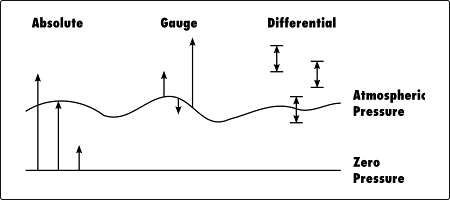
\includegraphics{img/pressure1.png} La relación entre las diferentes
presiones se puede escribir como

    \begin{Verbatim}[commandchars=\\\{\}]
{\color{incolor}In [{\color{incolor}1}]:} \PY{c}{\PYZpc{}\PYZpc{}latex}
        \PY{k}{\PYZbs{}begin}\PY{n+nb}{\PYZob{}}equation\PY{n+nb}{\PYZcb{}}
        p\PY{n+nb}{\PYZca{}}*(t) = p(t) \PYZhy{} p\PY{n+nb}{\PYZus{}}a
        \PY{k}{\PYZbs{}end}\PY{n+nb}{\PYZob{}}equation\PY{n+nb}{\PYZcb{}}
\end{Verbatim}


    \begin{equation}
p^*(t) = p(t) - p_a
\end{equation}

    
    donde \(p^*(t)\) representa la presión manométrica, \(p(t)\) la presión
absoluta y \(p_a\) la presión atmosférica. Una diferencia de presión,
denotada por \(\Delta p\), corresponde a la diferencia de presión entre
dos puntos.

    \subsection{3. Leyes de los elementos}\label{leyes-de-los-elementos}

Los sistemas hidráulicos poseen tres características que pueden
aproximarse por elementos concentrados: - Capacitancia (almacenamiento)
- Resistencia (oposición al flujo) - Inertancia (energía cinética del
fluido / despreciable respecto a las otras / no la consideraremos aquí.)

    \subsubsection{3.1 Capacitancia
Hidráulica}\label{capacitancia-hidruxe1ulica}

Cuando se almacena fluido en un contenedor abierto, existe una relación
algebráica entre el volumen del líquido y la presión en la base del
contenedor. Asumiendo \(A(h)\) como el area transversal del tanque,
\(h\) la altura del líquido, el volumen de líquido se puede escribir
como

    \begin{Verbatim}[commandchars=\\\{\}]
{\color{incolor}In [{\color{incolor}2}]:} \PY{c}{\PYZpc{}\PYZpc{}latex}
        \PY{k}{\PYZbs{}begin}\PY{n+nb}{\PYZob{}}equation\PY{n+nb}{\PYZcb{}}
            v = \PY{k}{\PYZbs{}int}\PY{n+nb}{\PYZus{}}0\PY{n+nb}{\PYZca{}}h A(\PY{k}{\PYZbs{}lambda}) d\PY{k}{\PYZbs{}lambda}
        \PY{k}{\PYZbs{}end}\PY{n+nb}{\PYZob{}}equation\PY{n+nb}{\PYZcb{}}
\end{Verbatim}


    \begin{equation}
    v = \int_0^h A(\lambda) d\lambda
\end{equation}

    
    La presión absoluta \(p\) y la altura \(h\) se encuentran relacionadas
como:

    \begin{Verbatim}[commandchars=\\\{\}]
{\color{incolor}In [{\color{incolor}3}]:} \PY{c}{\PYZpc{}\PYZpc{}latex}
        \PY{k}{\PYZbs{}begin}\PY{n+nb}{\PYZob{}}equation\PY{n+nb}{\PYZcb{}}
            p = \PY{k}{\PYZbs{}rho} g h + p\PY{n+nb}{\PYZus{}}a
        \PY{k}{\PYZbs{}end}\PY{n+nb}{\PYZob{}}equation\PY{n+nb}{\PYZcb{}}
\end{Verbatim}


    \begin{equation}
    p = \rho g h + p_a
\end{equation}

    
    donde \(\rho\) es la densidad del fluido y \(g\) la constante
gravitacional. Éstas dos ecuaciones implican que existe una única
relación algebráica entre la presión \(p\) y el volumen \(v\). Al
graficar la relación \emph{presión / volumen} para un tanque de sección
transversal constante se obtiene:

    \begin{figure}
\centering
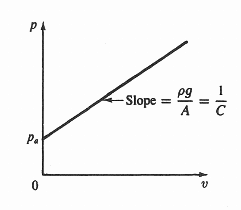
\includegraphics{img/capacitance_lin.png}
\caption{title}
\end{figure}

    y para un tanque de sección transversal variable se obtiene:

    \begin{figure}
\centering
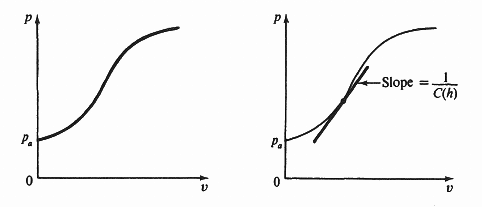
\includegraphics{img/capacitance.png}
\caption{title}
\end{figure}

    Al inverso de la pendiente de la recta tangente en algún punto de la
curva se define como \textbf{capacitancia hidráulica}, y se denota como
\(C(h)\):

    \begin{Verbatim}[commandchars=\\\{\}]
{\color{incolor}In [{\color{incolor}4}]:} \PY{c}{\PYZpc{}\PYZpc{}latex}
        \PY{k}{\PYZbs{}begin}\PY{n+nb}{\PYZob{}}equation\PY{n+nb}{\PYZcb{}}
            C(h) = \PY{k}{\PYZbs{}frac}\PY{n+nb}{\PYZob{}}1\PY{n+nb}{\PYZcb{}}\PY{n+nb}{\PYZob{}}dp/dv\PY{n+nb}{\PYZcb{}} = \PY{k}{\PYZbs{}frac}\PY{n+nb}{\PYZob{}}dv\PY{n+nb}{\PYZcb{}}\PY{n+nb}{\PYZob{}}dp\PY{n+nb}{\PYZcb{}}
        \PY{k}{\PYZbs{}end}\PY{n+nb}{\PYZob{}}equation\PY{n+nb}{\PYZcb{}}
\end{Verbatim}


    \begin{equation}
    C(h) = \frac{1}{dp/dv} = \frac{dv}{dp}
\end{equation}

    
    De la regla de la cadena de la derivada:

    \begin{Verbatim}[commandchars=\\\{\}]
{\color{incolor}In [{\color{incolor}5}]:} \PY{c}{\PYZpc{}\PYZpc{}latex}
        \PY{k}{\PYZbs{}begin}\PY{n+nb}{\PYZob{}}equation\PY{n+nb}{\PYZcb{}}
            C(h) = \PY{k}{\PYZbs{}frac}\PY{n+nb}{\PYZob{}}dv\PY{n+nb}{\PYZcb{}}\PY{n+nb}{\PYZob{}}dh\PY{n+nb}{\PYZcb{}} \PY{k}{\PYZbs{}frac}\PY{n+nb}{\PYZob{}}dh\PY{n+nb}{\PYZcb{}}\PY{n+nb}{\PYZob{}}dp\PY{n+nb}{\PYZcb{}}
        \PY{k}{\PYZbs{}end}\PY{n+nb}{\PYZob{}}equation\PY{n+nb}{\PYZcb{}}
\end{Verbatim}


    \begin{equation}
    C(h) = \frac{dv}{dh} \frac{dh}{dp}
\end{equation}

    
    De la segunda ecuación se sabe que \(dv/dh = A(h)\) y de la tercera que
\(dh/dp = 1/\rho g\). Por lo tanto, para un tanque de forma arbitraria:

    \begin{Verbatim}[commandchars=\\\{\}]
{\color{incolor}In [{\color{incolor}6}]:} \PY{c}{\PYZpc{}\PYZpc{}latex}
        \PY{k}{\PYZbs{}begin}\PY{n+nb}{\PYZob{}}equation\PY{n+nb}{\PYZcb{}}
            C(h) = \PY{k}{\PYZbs{}frac}\PY{n+nb}{\PYZob{}}A(h)\PY{n+nb}{\PYZcb{}}\PY{n+nb}{\PYZob{}}\PY{k}{\PYZbs{}rho} g\PY{n+nb}{\PYZcb{}}
        \PY{k}{\PYZbs{}end}\PY{n+nb}{\PYZob{}}equation\PY{n+nb}{\PYZcb{}}
\end{Verbatim}


    \begin{equation}
    C(h) = \frac{A(h)}{\rho g}
\end{equation}

    
    Para un tanque de sección constante \(A\), la segunda ecuación se reduce
a \(v = Ah\). Reemplazando en la tercera ecuación se tiene la presión en
términos del volumen:

    \begin{Verbatim}[commandchars=\\\{\}]
{\color{incolor}In [{\color{incolor}7}]:} \PY{c}{\PYZpc{}\PYZpc{}latex}
        \PY{k}{\PYZbs{}begin}\PY{n+nb}{\PYZob{}}equation\PY{n+nb}{\PYZcb{}}
            p = \PY{k}{\PYZbs{}frac}\PY{n+nb}{\PYZob{}}\PY{k}{\PYZbs{}rho} g\PY{n+nb}{\PYZcb{}}\PY{n+nb}{\PYZob{}}A\PY{n+nb}{\PYZcb{}}v + p\PY{n+nb}{\PYZus{}}a
        \PY{k}{\PYZbs{}end}\PY{n+nb}{\PYZob{}}equation\PY{n+nb}{\PYZcb{}}
\end{Verbatim}


    \begin{equation}
    p = \frac{\rho g}{A}v + p_a
\end{equation}

    
    que corresponde a la relación lineal mostrada en la segunda gráfica. El
volumen de líquido en un tanque en cualquier instante de tiempo
corresponde a la integral del flujo neto más el volumen inicial:

    \begin{Verbatim}[commandchars=\\\{\}]
{\color{incolor}In [{\color{incolor}8}]:} \PY{c}{\PYZpc{}\PYZpc{}latex}
        \PY{k}{\PYZbs{}begin}\PY{n+nb}{\PYZob{}}equation\PY{n+nb}{\PYZcb{}}
            v(t) = v(0) + \PY{k}{\PYZbs{}int}\PY{n+nb}{\PYZus{}}0\PY{n+nb}{\PYZca{}}t [w\PY{n+nb}{\PYZus{}}\PY{n+nb}{\PYZob{}}in\PY{n+nb}{\PYZcb{}}(\PY{k}{\PYZbs{}tau}) \PYZhy{} w\PY{n+nb}{\PYZus{}}\PY{n+nb}{\PYZob{}}out\PY{n+nb}{\PYZcb{}}(\PY{k}{\PYZbs{}tau})] d\PY{k}{\PYZbs{}tau}
        \PY{k}{\PYZbs{}end}\PY{n+nb}{\PYZob{}}equation\PY{n+nb}{\PYZcb{}}
\end{Verbatim}


    \begin{equation}
    v(t) = v(0) + \int_0^t [w_{in}(\tau) - w_{out}(\tau)] d\tau
\end{equation}

    
    Derivando ésta ecuación se puede obtener la forma alternativa:

    \begin{Verbatim}[commandchars=\\\{\}]
{\color{incolor}In [{\color{incolor}9}]:} \PY{c}{\PYZpc{}\PYZpc{}latex}
        \PY{k}{\PYZbs{}begin}\PY{n+nb}{\PYZob{}}equation\PY{n+nb}{\PYZcb{}}
            \PY{k}{\PYZbs{}dot}\PY{n+nb}{\PYZob{}}v\PY{n+nb}{\PYZcb{}} = w\PY{n+nb}{\PYZus{}}\PY{n+nb}{\PYZob{}}in\PY{n+nb}{\PYZcb{}}(t) \PYZhy{} w\PY{n+nb}{\PYZus{}}\PY{n+nb}{\PYZob{}}out\PY{n+nb}{\PYZcb{}}(t)
        \PY{k}{\PYZbs{}end}\PY{n+nb}{\PYZob{}}equation\PY{n+nb}{\PYZcb{}}
\end{Verbatim}


    \begin{equation}
    \dot{v} = w_{in}(t) - w_{out}(t)
\end{equation}

    
    Usando la regla de la cadena podemos escribir

    \begin{Verbatim}[commandchars=\\\{\}]
{\color{incolor}In [{\color{incolor}10}]:} \PY{c}{\PYZpc{}\PYZpc{}latex}
         \PY{k}{\PYZbs{}begin}\PY{n+nb}{\PYZob{}}equation\PY{n+nb}{\PYZcb{}}
             \PY{k}{\PYZbs{}frac}\PY{n+nb}{\PYZob{}}dv\PY{n+nb}{\PYZcb{}}\PY{n+nb}{\PYZob{}}dt\PY{n+nb}{\PYZcb{}} = \PY{k}{\PYZbs{}frac}\PY{n+nb}{\PYZob{}}dv\PY{n+nb}{\PYZcb{}}\PY{n+nb}{\PYZob{}}dh\PY{n+nb}{\PYZcb{}} \PY{k}{\PYZbs{}frac}\PY{n+nb}{\PYZob{}}dh\PY{n+nb}{\PYZcb{}}\PY{n+nb}{\PYZob{}}dt\PY{n+nb}{\PYZcb{}}
         \PY{k}{\PYZbs{}end}\PY{n+nb}{\PYZob{}}equation\PY{n+nb}{\PYZcb{}}
\end{Verbatim}


    \begin{equation}
    \frac{dv}{dt} = \frac{dv}{dh} \frac{dh}{dt}
\end{equation}

    
    Reemplazando \(dv/dh = A(h)\) en ésta última ecuación obtenemos

    \begin{Verbatim}[commandchars=\\\{\}]
{\color{incolor}In [{\color{incolor}11}]:} \PY{c}{\PYZpc{}\PYZpc{}latex}
         \PY{k}{\PYZbs{}begin}\PY{n+nb}{\PYZob{}}equation\PY{n+nb}{\PYZcb{}}
             \PY{k}{\PYZbs{}dot}\PY{n+nb}{\PYZob{}}h\PY{n+nb}{\PYZcb{}} = \PY{k}{\PYZbs{}frac}\PY{n+nb}{\PYZob{}}1\PY{n+nb}{\PYZcb{}}\PY{n+nb}{\PYZob{}}A(h)\PY{n+nb}{\PYZcb{}} [w\PY{n+nb}{\PYZus{}}\PY{n+nb}{\PYZob{}}in\PY{n+nb}{\PYZcb{}}(t) \PYZhy{} w\PY{n+nb}{\PYZus{}}\PY{n+nb}{\PYZob{}}out\PY{n+nb}{\PYZcb{}}(t)]
         \PY{k}{\PYZbs{}end}\PY{n+nb}{\PYZob{}}equation\PY{n+nb}{\PYZcb{}}
\end{Verbatim}


    \begin{equation}
    \dot{h} = \frac{1}{A(h)} [w_{in}(t) - w_{out}(t)]
\end{equation}

    
    De forma alternativa, se puede escribir \(dv/dt\) como

    \begin{Verbatim}[commandchars=\\\{\}]
{\color{incolor}In [{\color{incolor}12}]:} \PY{c}{\PYZpc{}\PYZpc{}latex}
         \PY{k}{\PYZbs{}begin}\PY{n+nb}{\PYZob{}}equation\PY{n+nb}{\PYZcb{}}
             \PY{k}{\PYZbs{}frac}\PY{n+nb}{\PYZob{}}dv\PY{n+nb}{\PYZcb{}}\PY{n+nb}{\PYZob{}}dt\PY{n+nb}{\PYZcb{}} = \PY{k}{\PYZbs{}frac}\PY{n+nb}{\PYZob{}}dv\PY{n+nb}{\PYZcb{}}\PY{n+nb}{\PYZob{}}dp\PY{n+nb}{\PYZcb{}} \PY{k}{\PYZbs{}frac}\PY{n+nb}{\PYZob{}}dp\PY{n+nb}{\PYZcb{}}\PY{n+nb}{\PYZob{}}dt\PY{n+nb}{\PYZcb{}}
         \PY{k}{\PYZbs{}end}\PY{n+nb}{\PYZob{}}equation\PY{n+nb}{\PYZcb{}}
\end{Verbatim}


    \begin{equation}
    \frac{dv}{dt} = \frac{dv}{dp} \frac{dp}{dt}
\end{equation}

    
    donde \(dv/dp = C(h)\). Por lo tanto se obtiene

    \begin{Verbatim}[commandchars=\\\{\}]
{\color{incolor}In [{\color{incolor}13}]:} \PY{c}{\PYZpc{}\PYZpc{}latex}
         \PY{k}{\PYZbs{}begin}\PY{n+nb}{\PYZob{}}equation\PY{n+nb}{\PYZcb{}}
             \PY{k}{\PYZbs{}dot}\PY{n+nb}{\PYZob{}}p\PY{n+nb}{\PYZcb{}} = \PY{k}{\PYZbs{}frac}\PY{n+nb}{\PYZob{}}1\PY{n+nb}{\PYZcb{}}\PY{n+nb}{\PYZob{}}C(h)\PY{n+nb}{\PYZcb{}} [w\PY{n+nb}{\PYZus{}}\PY{n+nb}{\PYZob{}}in\PY{n+nb}{\PYZcb{}}(t) \PYZhy{} w\PY{n+nb}{\PYZus{}}\PY{n+nb}{\PYZob{}}out\PY{n+nb}{\PYZcb{}}(t)] 
         \PY{k}{\PYZbs{}end}\PY{n+nb}{\PYZob{}}equation\PY{n+nb}{\PYZcb{}}
\end{Verbatim}


    \begin{equation}
    \dot{p} = \frac{1}{C(h)} [w_{in}(t) - w_{out}(t)] 
\end{equation}

    
    Cualquiera de las variables \(v\), \(h\) o \(p\) puede utilizarse para
representar la cantidad de líquido en un tanque, por lo que cualquiera
de éstas puede utilizarse como variable de estado. Si el área
transversal \(A(h)\) es variable, el modelo del sistema será no lineal.

    \subsubsection{Ejemplo 1:}\label{ejemplo-1}

Considere un tanque formado por un cilindro de radio \(R\) y longitud
\(L\) que contiene liquido de densidad \(\rho\). Encuentre la
capacitancia hidráulica cuando el tanque está ubicado de manera
vertical, y cuando está ubicado sobre el lado.

    \begin{figure}
\centering
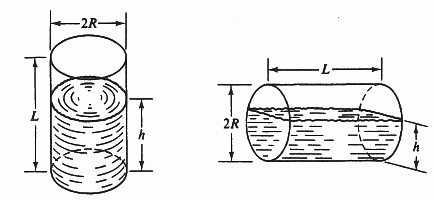
\includegraphics{img/cilinder_tank.png}
\caption{title}
\end{figure}

    \subsubsection{Solución:}\label{soluciuxf3n}

Para la primera configuración (vertical) el área transversal es
constante: \(A_1 =\pi R^2\). Por lo tanto, la capacitancia hidráulica
será \(C_1 = \pi R^2 / \rho g\). Para la segunda configuración
(horizontal) el área transversal depende de la altura \(h\). Dicha área
corresponde a \(A_s(h) = 2 \sqrt{R^2 - (R-h)^2}\). Por lo tanto la
capacitancia hidráulica será
\(C_2(h) = \frac{2L}{\rho g}\sqrt{R^2 - (R-h)^2}\).

    \subsubsection{3.2 Resistencia
Hidráulica}\label{resistencia-hidruxe1ulica}

Dado que el líquido fluye a través de tuberías, existe una caída de
presión a lo largo de éstas. También se presentan caídas de presión
cuando fluye a través de una válvula o de un orificio. Dicho cambio de
presión produce disipación de energía. La siguiente figura representa un
esquema de una válvula:

    \begin{figure}
\centering
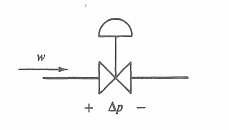
\includegraphics{img/valve.png}
\caption{title}
\end{figure}

    donde la flecha indica la dirección del flujo y los símbolos \(+\) y
\(-\) indican la caída de presión. La relación algebráica entre el flujo
volumétrico \(w\) y la diferencia de presión \(\Delta p\) se puede
escribir como

    \begin{Verbatim}[commandchars=\\\{\}]
{\color{incolor}In [{\color{incolor}14}]:} \PY{c}{\PYZpc{}\PYZpc{}latex}
         \PY{k}{\PYZbs{}begin}\PY{n+nb}{\PYZob{}}equation\PY{n+nb}{\PYZcb{}}
             w = k \PY{k}{\PYZbs{}sqrt}\PY{n+nb}{\PYZob{}}\PY{k}{\PYZbs{}Delta} p\PY{n+nb}{\PYZcb{}}
         \PY{k}{\PYZbs{}end}\PY{n+nb}{\PYZob{}}equation\PY{n+nb}{\PYZcb{}}
\end{Verbatim}


    \begin{equation}
    w = k \sqrt{\Delta p}
\end{equation}

    
    donde la constante \(k\) depende de las características de la tubería,
válvula u orificio. La siguiente figura presenta la forma típica de la
relación entre flujo volumétrico y diferencia de presión.

    \begin{figure}
\centering
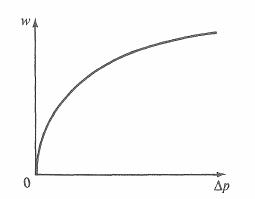
\includegraphics{img/valve_curve.png}
\caption{title}
\end{figure}

    Como ésta es una relación no lineal, es posible realizar una
linealizacion alrededor de un punto de operación, como se muestra en la
siguiente figura.

    \begin{figure}
\centering
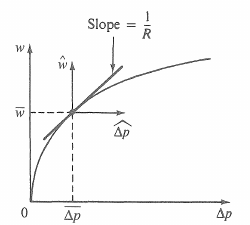
\includegraphics{img/valve_curve_linapprox.png}
\caption{title}
\end{figure}

    El inverso de la pendiente de la aproximación lineal se define como la
resistencia hidráulica \(R\). En éste caso tenemos

    \begin{Verbatim}[commandchars=\\\{\}]
{\color{incolor}In [{\color{incolor}15}]:} \PY{c}{\PYZpc{}\PYZpc{}latex}
         \PY{k}{\PYZbs{}begin}\PY{n+nb}{\PYZob{}}align\PY{n+nb}{\PYZcb{}}
             \PY{k}{\PYZbs{}frac}\PY{n+nb}{\PYZob{}}1\PY{n+nb}{\PYZcb{}}\PY{n+nb}{\PYZob{}}R\PY{n+nb}{\PYZcb{}} = \PY{k}{\PYZbs{}left}.\PY{k}{\PYZbs{}frac}\PY{n+nb}{\PYZob{}}dw\PY{n+nb}{\PYZcb{}}\PY{n+nb}{\PYZob{}}d \PY{k}{\PYZbs{}Delta} p\PY{n+nb}{\PYZcb{}}\PY{k}{\PYZbs{}right}|\PY{n+nb}{\PYZus{}}\PY{k}{\PYZbs{}bar}\PY{n+nb}{\PYZob{}}\PY{k}{\PYZbs{}Delta} p\PY{n+nb}{\PYZcb{}} \PY{n+nb}{\PYZam{}}= \PY{k}{\PYZbs{}left}.\PY{k}{\PYZbs{}frac}\PY{n+nb}{\PYZob{}}d\PY{n+nb}{\PYZcb{}}\PY{n+nb}{\PYZob{}}d \PY{k}{\PYZbs{}Delta} p\PY{n+nb}{\PYZcb{}} (k \PY{k}{\PYZbs{}Delta} p\PY{n+nb}{\PYZca{}}\PY{n+nb}{\PYZob{}}1/2)\PY{n+nb}{\PYZcb{}}) \PY{k}{\PYZbs{}right}|\PY{n+nb}{\PYZus{}}\PY{k}{\PYZbs{}bar}\PY{n+nb}{\PYZob{}}\PY{k}{\PYZbs{}Delta} p\PY{n+nb}{\PYZcb{}} = \PY{k}{\PYZbs{}frac}\PY{n+nb}{\PYZob{}}k\PY{n+nb}{\PYZcb{}}\PY{n+nb}{\PYZob{}}2\PY{k}{\PYZbs{}sqrt}\PY{n+nb}{\PYZob{}}\PY{k}{\PYZbs{}bar}\PY{n+nb}{\PYZob{}}\PY{k}{\PYZbs{}Delta} p\PY{n+nb}{\PYZcb{}}\PY{n+nb}{\PYZcb{}}\PY{n+nb}{\PYZcb{}}\PY{k}{\PYZbs{}\PYZbs{}}
             R \PY{n+nb}{\PYZam{}}= \PY{k}{\PYZbs{}frac}\PY{n+nb}{\PYZob{}}2\PY{k}{\PYZbs{}sqrt}\PY{n+nb}{\PYZob{}}\PY{k}{\PYZbs{}bar}\PY{n+nb}{\PYZob{}}\PY{k}{\PYZbs{}Delta} p\PY{n+nb}{\PYZcb{}}\PY{n+nb}{\PYZcb{}}\PY{n+nb}{\PYZcb{}}\PY{n+nb}{\PYZob{}}k\PY{n+nb}{\PYZcb{}}
         \PY{k}{\PYZbs{}end}\PY{n+nb}{\PYZob{}}align\PY{n+nb}{\PYZcb{}}
\end{Verbatim}


    \begin{align}
    \frac{1}{R} = \left.\frac{dw}{d \Delta p}\right|_\bar{\Delta p} &= \left.\frac{d}{d \Delta p} (k \Delta p^{1/2)}) \right|_\bar{\Delta p} = \frac{k}{2\sqrt{\bar{\Delta p}}}\\
    R &= \frac{2\sqrt{\bar{\Delta p}}}{k}
\end{align}

    
    Substituyendo \(\bar{w} = k \sqrt{\bar{\Delta p}}\) se obtiene una
expresión alternativa para la resistencia:

    \begin{Verbatim}[commandchars=\\\{\}]
{\color{incolor}In [{\color{incolor}16}]:} \PY{c}{\PYZpc{}\PYZpc{}latex}
         \PY{k}{\PYZbs{}begin}\PY{n+nb}{\PYZob{}}equation\PY{n+nb}{\PYZcb{}}
             R = \PY{k}{\PYZbs{}frac}\PY{n+nb}{\PYZob{}}2 \PY{k}{\PYZbs{}bar}\PY{n+nb}{\PYZob{}}w\PY{n+nb}{\PYZcb{}}\PY{n+nb}{\PYZcb{}}\PY{n+nb}{\PYZob{}}k\PY{n+nb}{\PYZca{}}2\PY{n+nb}{\PYZcb{}}
         \PY{k}{\PYZbs{}end}\PY{n+nb}{\PYZob{}}equation\PY{n+nb}{\PYZcb{}}
\end{Verbatim}


    \begin{equation}
    R = \frac{2 \bar{w}}{k^2}
\end{equation}

    
    \subsubsection{Ejemplo 2:}\label{ejemplo-2}

Encuentre el equivalente serie de dos válvulas conectadas en serie.

    \begin{figure}
\centering
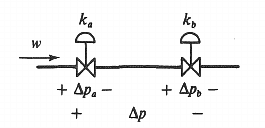
\includegraphics{img/valve_series.png}
\caption{title}
\end{figure}

    \subsubsection{Solución:}\label{soluciuxf3n}

Como están conectadas en serie, ambas válvulas tienen el mismo flujo
\(w\). La caída total de presión es

    \begin{Verbatim}[commandchars=\\\{\}]
{\color{incolor}In [{\color{incolor}17}]:} \PY{c}{\PYZpc{}\PYZpc{}latex}
         \PY{k}{\PYZbs{}begin}\PY{n+nb}{\PYZob{}}equation\PY{n+nb}{\PYZcb{}}
             \PY{k}{\PYZbs{}Delta} p = \PY{k}{\PYZbs{}Delta} p\PY{n+nb}{\PYZus{}}a + \PY{k}{\PYZbs{}Delta} p\PY{n+nb}{\PYZus{}}b = \PY{k}{\PYZbs{}left}(\PY{k}{\PYZbs{}frac}\PY{n+nb}{\PYZob{}}1\PY{n+nb}{\PYZcb{}}\PY{n+nb}{\PYZob{}}k\PY{n+nb}{\PYZus{}}a\PY{n+nb}{\PYZca{}}2\PY{n+nb}{\PYZcb{}} + \PY{k}{\PYZbs{}frac}\PY{n+nb}{\PYZob{}}1\PY{n+nb}{\PYZcb{}}\PY{n+nb}{\PYZob{}}k\PY{n+nb}{\PYZus{}}b\PY{n+nb}{\PYZca{}}2\PY{n+nb}{\PYZcb{}} \PY{k}{\PYZbs{}right}) w\PY{n+nb}{\PYZca{}}2
         \PY{k}{\PYZbs{}end}\PY{n+nb}{\PYZob{}}equation\PY{n+nb}{\PYZcb{}}
\end{Verbatim}


    \begin{equation}
    \Delta p = \Delta p_a + \Delta p_b = \left(\frac{1}{k_a^2} + \frac{1}{k_b^2} \right) w^2
\end{equation}

    
    Reorganizando los términos se obtiene:

    \begin{Verbatim}[commandchars=\\\{\}]
{\color{incolor}In [{\color{incolor}18}]:} \PY{c}{\PYZpc{}\PYZpc{}latex}
         \PY{k}{\PYZbs{}begin}\PY{n+nb}{\PYZob{}}equation\PY{n+nb}{\PYZcb{}}
             w = \PY{k}{\PYZbs{}left}(\PY{k}{\PYZbs{}frac}\PY{n+nb}{\PYZob{}}k\PY{n+nb}{\PYZus{}}a k\PY{n+nb}{\PYZus{}}b\PY{n+nb}{\PYZcb{}}\PY{n+nb}{\PYZob{}}\PY{k}{\PYZbs{}sqrt}\PY{n+nb}{\PYZob{}}k\PY{n+nb}{\PYZus{}}a\PY{n+nb}{\PYZca{}}2 + k\PY{n+nb}{\PYZus{}}b\PY{n+nb}{\PYZca{}}2\PY{n+nb}{\PYZcb{}}\PY{n+nb}{\PYZcb{}} \PY{k}{\PYZbs{}right}) \PY{k}{\PYZbs{}sqrt}\PY{n+nb}{\PYZob{}}\PY{k}{\PYZbs{}Delta} p\PY{n+nb}{\PYZcb{}} = k\PY{n+nb}{\PYZus{}}c \PY{k}{\PYZbs{}sqrt}\PY{n+nb}{\PYZob{}}\PY{k}{\PYZbs{}Delta} p\PY{n+nb}{\PYZcb{}}
         \PY{k}{\PYZbs{}end}\PY{n+nb}{\PYZob{}}equation\PY{n+nb}{\PYZcb{}}
\end{Verbatim}


    \begin{equation}
    w = \left(\frac{k_a k_b}{\sqrt{k_a^2 + k_b^2}} \right) \sqrt{\Delta p} = k_c \sqrt{\Delta p}
\end{equation}

    
    Ahora, para encontrar el equivalente lineal alrededor de un punto de
operacion se tiene:

    \begin{Verbatim}[commandchars=\\\{\}]
{\color{incolor}In [{\color{incolor}19}]:} \PY{c}{\PYZpc{}\PYZpc{}latex}
         \PY{k}{\PYZbs{}begin}\PY{n+nb}{\PYZob{}}equation\PY{n+nb}{\PYZcb{}}
             R\PY{n+nb}{\PYZus{}}c = \PY{k}{\PYZbs{}frac}\PY{n+nb}{\PYZob{}}2\PY{k}{\PYZbs{}bar}\PY{n+nb}{\PYZob{}}w\PY{n+nb}{\PYZcb{}}\PY{n+nb}{\PYZcb{}}\PY{n+nb}{\PYZob{}}k\PY{n+nb}{\PYZus{}}c\PY{n+nb}{\PYZca{}}2\PY{n+nb}{\PYZcb{}} = 2\PY{k}{\PYZbs{}bar}\PY{n+nb}{\PYZob{}}w\PY{n+nb}{\PYZcb{}} \PY{k}{\PYZbs{}left}(\PY{k}{\PYZbs{}frac}\PY{n+nb}{\PYZob{}}1\PY{n+nb}{\PYZcb{}}\PY{n+nb}{\PYZob{}}k\PY{n+nb}{\PYZus{}}a\PY{n+nb}{\PYZca{}}2\PY{n+nb}{\PYZcb{}} + \PY{k}{\PYZbs{}frac}\PY{n+nb}{\PYZob{}}1\PY{n+nb}{\PYZcb{}}\PY{n+nb}{\PYZob{}}k\PY{n+nb}{\PYZus{}}b\PY{n+nb}{\PYZca{}}2\PY{n+nb}{\PYZcb{}} \PY{k}{\PYZbs{}right}) = R\PY{n+nb}{\PYZus{}}a + R\PY{n+nb}{\PYZus{}}b
         \PY{k}{\PYZbs{}end}\PY{n+nb}{\PYZob{}}equation\PY{n+nb}{\PYZcb{}}
\end{Verbatim}


    \begin{equation}
    R_c = \frac{2\bar{w}}{k_c^2} = 2\bar{w} \left(\frac{1}{k_a^2} + \frac{1}{k_b^2} \right) = R_a + R_b
\end{equation}

    
    Por lo tanto, se observa que el equivalente serie de dos resistencias
hidráulicas corresponde a la suma de éstas.

    \subsubsection{3.3 Fuentes hidráulicas}\label{fuentes-hidruxe1ulicas}

En la mayoría de sistemas hidráulicos, la fuente de energía es una bomba
que obtiene su energía de un motor eléctrico. A continuación
consideraremos una bomba centrífuga controlada a velocidad constante. Su
representación gráfica se muestra en la siguiente figura:

    \begin{figure}
\centering
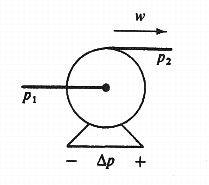
\includegraphics{img/pump.png}
\caption{title}
\end{figure}

    Las curvas típicas \emph{flujo / caída de presión} en una válvula se
muestran en la siguiente figura, para tres velocidades diferentes:

    \begin{figure}
\centering
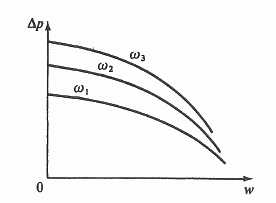
\includegraphics{img/pump_curves.png}
\caption{title}
\end{figure}

    Dichas curvas se obtienen de manera experimental para condiciones
estacionarias. Como puede observarse, dichas relaciones también son no
lineales. En éste caso también es posible encontrar una aproximación
lineal dado un punto de operación, como se muestra en la siguiente
figura:

    \begin{figure}
\centering
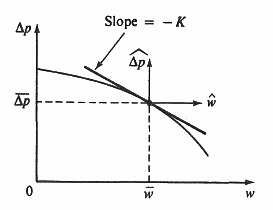
\includegraphics{img/pump_linapprox.png}
\caption{title}
\end{figure}

    La expansión en serie de Taylor del flujo \(w\) en función de la
diferencia de presión es:

    \begin{Verbatim}[commandchars=\\\{\}]
{\color{incolor}In [{\color{incolor}20}]:} \PY{c}{\PYZpc{}\PYZpc{}latex}
         \PY{k}{\PYZbs{}begin}\PY{n+nb}{\PYZob{}}equation\PY{n+nb}{\PYZcb{}}
             w = \PY{k}{\PYZbs{}bar}\PY{n+nb}{\PYZob{}}w\PY{n+nb}{\PYZcb{}} + \PY{k}{\PYZbs{}left}.\PY{k}{\PYZbs{}frac}\PY{n+nb}{\PYZob{}}dw\PY{n+nb}{\PYZcb{}}\PY{n+nb}{\PYZob{}}d \PY{k}{\PYZbs{}Delta} p\PY{n+nb}{\PYZcb{}}\PY{k}{\PYZbs{}right}|\PY{n+nb}{\PYZus{}}\PY{n+nb}{\PYZob{}}\PY{k}{\PYZbs{}bar}\PY{n+nb}{\PYZob{}}\PY{k}{\PYZbs{}Delta} p\PY{n+nb}{\PYZcb{}}\PY{n+nb}{\PYZcb{}} (\PY{k}{\PYZbs{}Delta} p \PYZhy{} \PY{k}{\PYZbs{}bar}\PY{n+nb}{\PYZob{}}\PY{k}{\PYZbs{}Delta} p\PY{n+nb}{\PYZcb{}}) + \PY{k}{\PYZbs{}dots}
         \PY{k}{\PYZbs{}end}\PY{n+nb}{\PYZob{}}equation\PY{n+nb}{\PYZcb{}}
\end{Verbatim}


    \begin{equation}
    w = \bar{w} + \left.\frac{dw}{d \Delta p}\right|_{\bar{\Delta p}} (\Delta p - \bar{\Delta p}) + \dots
\end{equation}

    
    Tomando los dos primeros términos de la serie se obtiene la aproximación
lineal, donde la relación para las variables incrementales es:

    \begin{Verbatim}[commandchars=\\\{\}]
{\color{incolor}In [{\color{incolor}21}]:} \PY{c}{\PYZpc{}\PYZpc{}latex}
         \PY{k}{\PYZbs{}begin}\PY{n+nb}{\PYZob{}}equation\PY{n+nb}{\PYZcb{}}
             \PY{k}{\PYZbs{}hat}\PY{n+nb}{\PYZob{}}w\PY{n+nb}{\PYZcb{}} = \PYZhy{}\PY{k}{\PYZbs{}frac}\PY{n+nb}{\PYZob{}}1\PY{n+nb}{\PYZcb{}}\PY{n+nb}{\PYZob{}}K\PY{n+nb}{\PYZcb{}} \PY{k}{\PYZbs{}hat}\PY{n+nb}{\PYZob{}}\PY{k}{\PYZbs{}Delta} p\PY{n+nb}{\PYZcb{}}
         \PY{k}{\PYZbs{}end}\PY{n+nb}{\PYZob{}}equation\PY{n+nb}{\PYZcb{}}
\end{Verbatim}


    \begin{equation}
    \hat{w} = -\frac{1}{K} \hat{\Delta p}
\end{equation}

    
    \subsection{4. Modelos Dinámicos de Sistemas
Hidráulicos}\label{modelos-dinuxe1micos-de-sistemas-hidruxe1ulicos}

En ésta sección se desarrollarán los modelos de sistemas a partir de las
leyes de los elementos que los componen, y de las leyes de
interconexión.

    \subsubsection{Ejemplo 3:}\label{ejemplo-3}

Para el sistema hidráulico mostrado en la figura:
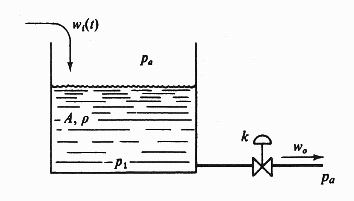
\includegraphics{img/tank_valve.png} - Formule el modelo matemático. -
Obtenga el punto de operación. - Obtenga el modelo linealizado alrededor
del punto de operación, para una entrada \(\bar{w}_i\). - Simule la
respuesta del sistema ante una entrada paso de amplitud
\(\bar{w}_i = 5 \times 10^{-3}\), asumiendo como condición inicial que
el tanque está vacio. Los valores de los parámetros son \(A=2\),
\(\rho=1000\), \(k = 5 \times 10^{-5}\), \(p_a = 1.013 \times 10^{5}\),
\(g = 9.807\).

    \subsubsection{Solución:}\label{soluciuxf3n}

\begin{itemize}
\tightlist
\item
  Tomando la presión \(p_1\) como variable de estado, podemos escribir
  la ecuación dinámica para el tanque como:
\end{itemize}

    \begin{Verbatim}[commandchars=\\\{\}]
{\color{incolor}In [{\color{incolor}22}]:} \PY{c}{\PYZpc{}\PYZpc{}latex}
         \PY{k}{\PYZbs{}begin}\PY{n+nb}{\PYZob{}}equation\PY{n+nb}{\PYZcb{}}
             \PY{k}{\PYZbs{}dot}\PY{n+nb}{\PYZob{}}p\PY{n+nb}{\PYZcb{}}\PY{n+nb}{\PYZus{}}1(t) = \PY{k}{\PYZbs{}frac}\PY{n+nb}{\PYZob{}}1\PY{n+nb}{\PYZcb{}}\PY{n+nb}{\PYZob{}}C\PY{n+nb}{\PYZcb{}} [w\PY{n+nb}{\PYZus{}}\PY{n+nb}{\PYZob{}}in\PY{n+nb}{\PYZcb{}}(t) \PYZhy{} w\PY{n+nb}{\PYZus{}}\PY{n+nb}{\PYZob{}}out\PY{n+nb}{\PYZcb{}}(t)]
         \PY{k}{\PYZbs{}end}\PY{n+nb}{\PYZob{}}equation\PY{n+nb}{\PYZcb{}}
\end{Verbatim}


    \begin{equation}
    \dot{p}_1(t) = \frac{1}{C} [w_{in}(t) - w_{out}(t)]
\end{equation}

    
    donde \(w_{in}(t) = w_i(t)\) and \(w_{out}(t) = k \sqrt{p_1(t) - p_a}\).
Sustituyendo se obtiene:

    \begin{Verbatim}[commandchars=\\\{\}]
{\color{incolor}In [{\color{incolor}23}]:} \PY{c}{\PYZpc{}\PYZpc{}latex}
         \PY{k}{\PYZbs{}begin}\PY{n+nb}{\PYZob{}}equation\PY{n+nb}{\PYZcb{}}
             \PY{k}{\PYZbs{}dot}\PY{n+nb}{\PYZob{}}p\PY{n+nb}{\PYZcb{}}\PY{n+nb}{\PYZus{}}1(t) = \PY{k}{\PYZbs{}frac}\PY{n+nb}{\PYZob{}}\PY{k}{\PYZbs{}rho} g\PY{n+nb}{\PYZcb{}}\PY{n+nb}{\PYZob{}}A\PY{n+nb}{\PYZcb{}} [w\PY{n+nb}{\PYZus{}}i(t) \PYZhy{} k \PY{k}{\PYZbs{}sqrt}\PY{n+nb}{\PYZob{}}p\PY{n+nb}{\PYZus{}}1(t) \PYZhy{} p\PY{n+nb}{\PYZus{}}a\PY{n+nb}{\PYZcb{}}]
         \PY{k}{\PYZbs{}end}\PY{n+nb}{\PYZob{}}equation\PY{n+nb}{\PYZcb{}}
\end{Verbatim}


    \begin{equation}
    \dot{p}_1(t) = \frac{\rho g}{A} [w_i(t) - k \sqrt{p_1(t) - p_a}]
\end{equation}

    
    \begin{itemize}
\tightlist
\item
  Para encontrar el punto de operación se hace \(\dot{p}_1 = 0\), y se
  despeja \(\bar{p}_1\).
\end{itemize}

    \begin{Verbatim}[commandchars=\\\{\}]
{\color{incolor}In [{\color{incolor}24}]:} \PY{c}{\PYZpc{}\PYZpc{}latex}
         \PY{k}{\PYZbs{}begin}\PY{n+nb}{\PYZob{}}align\PY{n+nb}{\PYZcb{}}
             0 \PY{n+nb}{\PYZam{}}= \PY{k}{\PYZbs{}frac}\PY{n+nb}{\PYZob{}}\PY{k}{\PYZbs{}rho} g\PY{n+nb}{\PYZcb{}}\PY{n+nb}{\PYZob{}}A\PY{n+nb}{\PYZcb{}} [\PY{k}{\PYZbs{}bar}\PY{n+nb}{\PYZob{}}w\PY{n+nb}{\PYZcb{}}\PY{n+nb}{\PYZus{}}i \PYZhy{} k \PY{k}{\PYZbs{}sqrt}\PY{n+nb}{\PYZob{}}\PY{k}{\PYZbs{}bar}\PY{n+nb}{\PYZob{}}p\PY{n+nb}{\PYZcb{}}\PY{n+nb}{\PYZus{}}1 \PYZhy{} p\PY{n+nb}{\PYZus{}}a\PY{n+nb}{\PYZcb{}}]\PY{k}{\PYZbs{}\PYZbs{}}
             \PY{k}{\PYZbs{}bar}\PY{n+nb}{\PYZob{}}w\PY{n+nb}{\PYZcb{}}\PY{n+nb}{\PYZus{}}i \PY{n+nb}{\PYZam{}}= k \PY{k}{\PYZbs{}sqrt}\PY{n+nb}{\PYZob{}}\PY{k}{\PYZbs{}bar}\PY{n+nb}{\PYZob{}}p\PY{n+nb}{\PYZcb{}}\PY{n+nb}{\PYZus{}}1 \PYZhy{} p\PY{n+nb}{\PYZus{}}a\PY{n+nb}{\PYZcb{}}\PY{k}{\PYZbs{}\PYZbs{}}
             \PY{k}{\PYZbs{}bar}\PY{n+nb}{\PYZob{}}p\PY{n+nb}{\PYZcb{}}\PY{n+nb}{\PYZus{}}1 \PY{n+nb}{\PYZam{}}= \PY{k}{\PYZbs{}frac}\PY{n+nb}{\PYZob{}}\PY{k}{\PYZbs{}bar}\PY{n+nb}{\PYZob{}}w\PY{n+nb}{\PYZcb{}}\PY{n+nb}{\PYZus{}}i\PY{n+nb}{\PYZca{}}2\PY{n+nb}{\PYZcb{}}\PY{n+nb}{\PYZob{}}k\PY{n+nb}{\PYZca{}}2\PY{n+nb}{\PYZcb{}} + p\PY{n+nb}{\PYZus{}}a
         \PY{k}{\PYZbs{}end}\PY{n+nb}{\PYZob{}}align\PY{n+nb}{\PYZcb{}}
\end{Verbatim}


    \begin{align}
    0 &= \frac{\rho g}{A} [\bar{w}_i - k \sqrt{\bar{p}_1 - p_a}]\\
    \bar{w}_i &= k \sqrt{\bar{p}_1 - p_a}\\
    \bar{p}_1 &= \frac{\bar{w}_i^2}{k^2} + p_a
\end{align}

    
    \begin{itemize}
\tightlist
\item
  Para obtener el modelo linealizado, calculamos las derivadas parciales
  (jacobiano) para obtener los coeficientes del modelo incremental:
\end{itemize}

    \begin{Verbatim}[commandchars=\\\{\}]
{\color{incolor}In [{\color{incolor}25}]:} \PY{c}{\PYZpc{}\PYZpc{}latex}
         \PY{k}{\PYZbs{}begin}\PY{n+nb}{\PYZob{}}align\PY{n+nb}{\PYZcb{}}
             \PY{k}{\PYZbs{}left}.\PY{k}{\PYZbs{}frac}\PY{n+nb}{\PYZob{}}\PY{k}{\PYZbs{}partial} f\PY{n+nb}{\PYZcb{}}\PY{n+nb}{\PYZob{}}\PY{k}{\PYZbs{}partial} p\PY{n+nb}{\PYZus{}}1\PY{n+nb}{\PYZcb{}}\PY{k}{\PYZbs{}right}|\PY{n+nb}{\PYZus{}}\PY{n+nb}{\PYZob{}}\PY{k}{\PYZbs{}bar}\PY{n+nb}{\PYZob{}}w\PY{n+nb}{\PYZcb{}}\PY{n+nb}{\PYZus{}}i,\PY{k}{\PYZbs{}bar}\PY{n+nb}{\PYZob{}}p\PY{n+nb}{\PYZcb{}}\PY{n+nb}{\PYZus{}}1\PY{n+nb}{\PYZcb{}} \PY{n+nb}{\PYZam{}}= \PY{k}{\PYZbs{}left}.\PYZhy{}\PY{k}{\PYZbs{}frac}\PY{n+nb}{\PYZob{}}\PY{k}{\PYZbs{}rho} g k\PY{n+nb}{\PYZcb{}}\PY{n+nb}{\PYZob{}}2A\PY{n+nb}{\PYZcb{}} (\PY{k}{\PYZbs{}bar}\PY{n+nb}{\PYZob{}}p\PY{n+nb}{\PYZcb{}}\PY{n+nb}{\PYZus{}}1\PYZhy{}p\PY{n+nb}{\PYZus{}}a)\PY{n+nb}{\PYZca{}}\PY{n+nb}{\PYZob{}}\PYZhy{}1/2\PY{n+nb}{\PYZcb{}}\PY{k}{\PYZbs{}right}|\PY{n+nb}{\PYZus{}}\PY{n+nb}{\PYZob{}}\PY{k}{\PYZbs{}bar}\PY{n+nb}{\PYZob{}}w\PY{n+nb}{\PYZcb{}}\PY{n+nb}{\PYZus{}}i,\PY{k}{\PYZbs{}bar}\PY{n+nb}{\PYZob{}}p\PY{n+nb}{\PYZcb{}}\PY{n+nb}{\PYZus{}}1\PY{n+nb}{\PYZcb{}}\PY{k}{\PYZbs{}\PYZbs{}}
             \PY{n+nb}{\PYZam{}}= \PYZhy{}\PY{k}{\PYZbs{}frac}\PY{n+nb}{\PYZob{}}\PY{k}{\PYZbs{}rho} g k\PY{n+nb}{\PYZcb{}}\PY{n+nb}{\PYZob{}}2A\PY{n+nb}{\PYZcb{}} \PY{k}{\PYZbs{}left}(\PY{k}{\PYZbs{}frac}\PY{n+nb}{\PYZob{}}\PY{k}{\PYZbs{}bar}\PY{n+nb}{\PYZob{}}w\PY{n+nb}{\PYZcb{}}\PY{n+nb}{\PYZus{}}i\PY{n+nb}{\PYZca{}}2\PY{n+nb}{\PYZcb{}}\PY{n+nb}{\PYZob{}}k\PY{n+nb}{\PYZca{}}2\PY{n+nb}{\PYZcb{}}+p\PY{n+nb}{\PYZus{}}a\PYZhy{}p\PY{n+nb}{\PYZus{}}a\PY{k}{\PYZbs{}right})\PY{n+nb}{\PYZca{}}\PY{n+nb}{\PYZob{}}\PYZhy{}1/2\PY{n+nb}{\PYZcb{}}\PY{k}{\PYZbs{}\PYZbs{}}
             \PY{n+nb}{\PYZam{}}= \PYZhy{}\PY{k}{\PYZbs{}frac}\PY{n+nb}{\PYZob{}}\PY{k}{\PYZbs{}rho} g k\PY{n+nb}{\PYZca{}}2\PY{n+nb}{\PYZcb{}}\PY{n+nb}{\PYZob{}}2A \PY{k}{\PYZbs{}bar}\PY{n+nb}{\PYZob{}}w\PY{n+nb}{\PYZcb{}}\PY{n+nb}{\PYZus{}}i\PY{n+nb}{\PYZcb{}}\PY{k}{\PYZbs{}\PYZbs{}}
             \PY{n+nb}{\PYZam{}}= \PYZhy{}\PY{k}{\PYZbs{}frac}\PY{n+nb}{\PYZob{}}1\PY{n+nb}{\PYZcb{}}\PY{n+nb}{\PYZob{}}RC\PY{n+nb}{\PYZcb{}}
         \PY{k}{\PYZbs{}end}\PY{n+nb}{\PYZob{}}align\PY{n+nb}{\PYZcb{}}
\end{Verbatim}


    \begin{align}
    \left.\frac{\partial f}{\partial p_1}\right|_{\bar{w}_i,\bar{p}_1} &= \left.-\frac{\rho g k}{2A} (\bar{p}_1-p_a)^{-1/2}\right|_{\bar{w}_i,\bar{p}_1}\\
    &= -\frac{\rho g k}{2A} \left(\frac{\bar{w}_i^2}{k^2}+p_a-p_a\right)^{-1/2}\\
    &= -\frac{\rho g k^2}{2A \bar{w}_i}\\
    &= -\frac{1}{RC}
\end{align}

    
    donde \(R=2\bar{w}_i/k^2\) y \(C = A/\rho g\). El siguiente coeficiente
es:

    \begin{Verbatim}[commandchars=\\\{\}]
{\color{incolor}In [{\color{incolor}26}]:} \PY{c}{\PYZpc{}\PYZpc{}latex}
         \PY{k}{\PYZbs{}begin}\PY{n+nb}{\PYZob{}}equation\PY{n+nb}{\PYZcb{}}
             \PY{k}{\PYZbs{}left}.\PY{k}{\PYZbs{}frac}\PY{n+nb}{\PYZob{}}\PY{k}{\PYZbs{}partial} f\PY{n+nb}{\PYZcb{}}\PY{n+nb}{\PYZob{}}\PY{k}{\PYZbs{}partial} w\PY{n+nb}{\PYZus{}}i\PY{n+nb}{\PYZcb{}}\PY{k}{\PYZbs{}right}|\PY{n+nb}{\PYZus{}}\PY{n+nb}{\PYZob{}}\PY{k}{\PYZbs{}bar}\PY{n+nb}{\PYZob{}}w\PY{n+nb}{\PYZcb{}}\PY{n+nb}{\PYZus{}}i,\PY{k}{\PYZbs{}bar}\PY{n+nb}{\PYZob{}}p\PY{n+nb}{\PYZcb{}}\PY{n+nb}{\PYZus{}}1\PY{n+nb}{\PYZcb{}} = \PY{k}{\PYZbs{}frac}\PY{n+nb}{\PYZob{}}\PY{k}{\PYZbs{}rho} g\PY{n+nb}{\PYZcb{}}\PY{n+nb}{\PYZob{}}A\PY{n+nb}{\PYZcb{}} = \PY{k}{\PYZbs{}frac}\PY{n+nb}{\PYZob{}}1\PY{n+nb}{\PYZcb{}}\PY{n+nb}{\PYZob{}}C\PY{n+nb}{\PYZcb{}}
         \PY{k}{\PYZbs{}end}\PY{n+nb}{\PYZob{}}equation\PY{n+nb}{\PYZcb{}}
\end{Verbatim}


    \begin{equation}
    \left.\frac{\partial f}{\partial w_i}\right|_{\bar{w}_i,\bar{p}_1} = \frac{\rho g}{A} = \frac{1}{C}
\end{equation}

    
    Entonces, el modelo linealizado es:

    \begin{Verbatim}[commandchars=\\\{\}]
{\color{incolor}In [{\color{incolor}27}]:} \PY{c}{\PYZpc{}\PYZpc{}latex}
         \PY{k}{\PYZbs{}begin}\PY{n+nb}{\PYZob{}}equation\PY{n+nb}{\PYZcb{}}
             \PY{k}{\PYZbs{}dot}\PY{n+nb}{\PYZob{}}\PY{k}{\PYZbs{}hat}\PY{n+nb}{\PYZob{}}p\PY{n+nb}{\PYZcb{}}\PY{n+nb}{\PYZcb{}}\PY{n+nb}{\PYZus{}}1 = \PYZhy{}\PY{k}{\PYZbs{}frac}\PY{n+nb}{\PYZob{}}1\PY{n+nb}{\PYZcb{}}\PY{n+nb}{\PYZob{}}RC\PY{n+nb}{\PYZcb{}} \PY{k}{\PYZbs{}hat}\PY{n+nb}{\PYZob{}}p\PY{n+nb}{\PYZcb{}}\PY{n+nb}{\PYZus{}}1 + \PY{k}{\PYZbs{}frac}\PY{n+nb}{\PYZob{}}1\PY{n+nb}{\PYZcb{}}\PY{n+nb}{\PYZob{}}C\PY{n+nb}{\PYZcb{}} \PY{k}{\PYZbs{}hat}\PY{n+nb}{\PYZob{}}w\PY{n+nb}{\PYZcb{}}\PY{n+nb}{\PYZus{}}i
         \PY{k}{\PYZbs{}end}\PY{n+nb}{\PYZob{}}equation\PY{n+nb}{\PYZcb{}}
\end{Verbatim}


    \begin{equation}
    \dot{\hat{p}}_1 = -\frac{1}{RC} \hat{p}_1 + \frac{1}{C} \hat{w}_i
\end{equation}

    
    \begin{itemize}
\tightlist
\item
  Para obtener la simulación del sistema escribiremos un script de
  Python, usando funciones de las librerías \texttt{numpy},
  \texttt{matplotlib} y \texttt{scipy}. En primer lugar, importamos las
  librerías necesarias y configuramos el entorno.
\end{itemize}

    \begin{Verbatim}[commandchars=\\\{\}]
{\color{incolor}In [{\color{incolor}42}]:} \PY{k+kn}{import} \PY{n+nn}{math}
         \PY{k+kn}{import} \PY{n+nn}{numpy} \PY{k}{as} \PY{n+nn}{np}
         \PY{o}{\PYZpc{}}\PY{k}{matplotlib} inline
         \PY{k+kn}{import} \PY{n+nn}{matplotlib}\PY{n+nn}{.}\PY{n+nn}{pyplot} \PY{k}{as} \PY{n+nn}{plt}
         \PY{k+kn}{import} \PY{n+nn}{matplotlib}
         \PY{n}{matplotlib}\PY{o}{.}\PY{n}{rcParams}\PY{p}{[}\PY{l+s+s1}{\PYZsq{}}\PY{l+s+s1}{lines.linewidth}\PY{l+s+s1}{\PYZsq{}}\PY{p}{]} \PY{o}{=} \PY{l+m+mi}{3}
         \PY{n}{matplotlib}\PY{o}{.}\PY{n}{rcParams}\PY{p}{[}\PY{l+s+s1}{\PYZsq{}}\PY{l+s+s1}{font.size}\PY{l+s+s1}{\PYZsq{}}\PY{p}{]} \PY{o}{=} \PY{l+m+mi}{13}
         \PY{n}{matplotlib}\PY{o}{.}\PY{n}{rcParams}\PY{p}{[}\PY{l+s+s1}{\PYZsq{}}\PY{l+s+s1}{lines.markersize}\PY{l+s+s1}{\PYZsq{}}\PY{p}{]} \PY{o}{=} \PY{l+m+mi}{5}
         \PY{n}{matplotlib}\PY{o}{.}\PY{n}{rcParams}\PY{p}{[}\PY{l+s+s1}{\PYZsq{}}\PY{l+s+s1}{figure.figsize}\PY{l+s+s1}{\PYZsq{}}\PY{p}{]} \PY{o}{=} \PY{p}{(}\PY{l+m+mi}{14}\PY{p}{,} \PY{l+m+mi}{9}\PY{p}{)}
         \PY{n}{matplotlib}\PY{o}{.}\PY{n}{rc}\PY{p}{(}\PY{l+s+s1}{\PYZsq{}}\PY{l+s+s1}{text}\PY{l+s+s1}{\PYZsq{}}\PY{p}{,} \PY{n}{usetex}\PY{o}{=}\PY{k+kc}{True}\PY{p}{)}
         \PY{n}{matplotlib}\PY{o}{.}\PY{n}{rc}\PY{p}{(}\PY{l+s+s1}{\PYZsq{}}\PY{l+s+s1}{axes}\PY{l+s+s1}{\PYZsq{}}\PY{p}{,} \PY{n}{grid} \PY{o}{=} \PY{k+kc}{False}\PY{p}{,} \PY{n}{labelsize}\PY{o}{=}\PY{l+m+mi}{14}\PY{p}{,} \PY{n}{titlesize}\PY{o}{=}\PY{l+m+mi}{16}\PY{p}{,} \PY{n}{ymargin}\PY{o}{=}\PY{l+m+mf}{0.05}\PY{p}{)}
         \PY{n}{matplotlib}\PY{o}{.}\PY{n}{rc}\PY{p}{(}\PY{l+s+s1}{\PYZsq{}}\PY{l+s+s1}{legend}\PY{l+s+s1}{\PYZsq{}}\PY{p}{,} \PY{n}{numpoints}\PY{o}{=}\PY{l+m+mi}{1}\PY{p}{,} \PY{n}{fontsize}\PY{o}{=}\PY{l+m+mi}{11}\PY{p}{)}
\end{Verbatim}


    Ahora definimos los parámetros del sistema.

    \begin{Verbatim}[commandchars=\\\{\}]
{\color{incolor}In [{\color{incolor}43}]:} \PY{n}{A} \PY{o}{=} \PY{l+m+mi}{2}
         \PY{n}{rho} \PY{o}{=} \PY{l+m+mi}{1000}
         \PY{n}{k} \PY{o}{=} \PY{l+m+mf}{5e\PYZhy{}5}
         \PY{n}{pa} \PY{o}{=} \PY{l+m+mf}{1.013e5}
         \PY{n}{g} \PY{o}{=} \PY{l+m+mf}{9.807}
         \PY{n}{wibar} \PY{o}{=} \PY{l+m+mf}{6e\PYZhy{}3}
\end{Verbatim}


    Implementamos una función de python correspondiente a la ecuación
dinámica del sistema:

    \begin{Verbatim}[commandchars=\\\{\}]
{\color{incolor}In [{\color{incolor}44}]:} \PY{k}{def} \PY{n+nf}{hydrsys\PYZus{}eq}\PY{p}{(}\PY{n}{t}\PY{p}{,} \PY{n}{p1}\PY{p}{)}\PY{p}{:}    
             \PY{n}{A} \PY{o}{=} \PY{l+m+mi}{2}
             \PY{n}{rho} \PY{o}{=} \PY{l+m+mi}{1000}
             \PY{n}{k} \PY{o}{=} \PY{l+m+mf}{5e\PYZhy{}5}
             \PY{n}{pa} \PY{o}{=} \PY{l+m+mf}{1.013e5}
             \PY{n}{g} \PY{o}{=} \PY{l+m+mf}{9.807}
             \PY{n}{wibar} \PY{o}{=} \PY{l+m+mf}{6e\PYZhy{}3}
             \PY{n}{pdot} \PY{o}{=} \PY{p}{(}\PY{n}{rho}\PY{o}{*}\PY{n}{g}\PY{p}{)}\PY{o}{/}\PY{n}{A} \PY{o}{*} \PY{p}{(}\PY{n}{wibar} \PY{o}{\PYZhy{}} \PY{n}{k}\PY{o}{*}\PY{n}{math}\PY{o}{.}\PY{n}{sqrt}\PY{p}{(}\PY{n}{p1} \PY{o}{\PYZhy{}} \PY{n}{pa}\PY{p}{)}\PY{p}{)}
             \PY{k}{return} \PY{n}{pdot}
\end{Verbatim}


    Ahora, implementamos el método iterativo de Runge-Kutta de dos etapas:

    \begin{Verbatim}[commandchars=\\\{\}]
{\color{incolor}In [{\color{incolor}45}]:} \PY{n}{tf} \PY{o}{=} \PY{l+m+mi}{10000}
         \PY{n}{N} \PY{o}{=} \PY{l+m+mi}{10000}
         \PY{n}{h} \PY{o}{=} \PY{n}{tf}\PY{o}{/}\PY{n}{N}
         \PY{n}{t} \PY{o}{=} \PY{n}{np}\PY{o}{.}\PY{n}{linspace}\PY{p}{(}\PY{l+m+mi}{0}\PY{p}{,}\PY{n}{tf}\PY{p}{,}\PY{n}{N}\PY{p}{)}
         \PY{n}{p1} \PY{o}{=} \PY{n}{np}\PY{o}{.}\PY{n}{zeros}\PY{p}{(}\PY{n}{N}\PY{p}{)}
         \PY{n}{p1}\PY{p}{[}\PY{l+m+mi}{0}\PY{p}{]} \PY{o}{=} \PY{n}{pa}
         \PY{k}{for} \PY{n}{i} \PY{o+ow}{in} \PY{n+nb}{range}\PY{p}{(}\PY{l+m+mi}{0}\PY{p}{,}\PY{n}{N}\PY{o}{\PYZhy{}}\PY{l+m+mi}{1}\PY{p}{)}\PY{p}{:}
             \PY{n}{k1} \PY{o}{=} \PY{n}{hydrsys\PYZus{}eq}\PY{p}{(}\PY{n}{t}\PY{p}{[}\PY{n}{i}\PY{p}{]}\PY{p}{,}\PY{n}{p1}\PY{p}{[}\PY{n}{i}\PY{p}{]}\PY{p}{)}
             \PY{n}{k2} \PY{o}{=} \PY{n}{hydrsys\PYZus{}eq}\PY{p}{(}\PY{n}{t}\PY{p}{[}\PY{n}{i}\PY{p}{]}\PY{o}{+}\PY{l+m+mf}{0.5}\PY{o}{*}\PY{n}{h}\PY{p}{,}\PY{n}{p1}\PY{p}{[}\PY{n}{i}\PY{p}{]}\PY{o}{+}\PY{l+m+mf}{0.5}\PY{o}{*}\PY{n}{h}\PY{o}{*}\PY{n}{k1}\PY{p}{)}
             \PY{n}{p1}\PY{p}{[}\PY{n}{i}\PY{o}{+}\PY{l+m+mi}{1}\PY{p}{]} \PY{o}{=} \PY{n}{p1}\PY{p}{[}\PY{n}{i}\PY{p}{]} \PY{o}{+} \PY{n}{h}\PY{o}{*}\PY{n}{k2}
\end{Verbatim}


    Finalmente graficamos la respuesta:

    \begin{Verbatim}[commandchars=\\\{\}]
{\color{incolor}In [{\color{incolor}47}]:} \PY{n}{p1bar} \PY{o}{=} \PY{n}{wibar}\PY{o}{*}\PY{o}{*}\PY{l+m+mi}{2}\PY{o}{/}\PY{n}{k}\PY{o}{*}\PY{o}{*}\PY{l+m+mi}{2} \PY{o}{+} \PY{n}{pa}
         \PY{n}{p1bar} \PY{o}{=} \PY{n}{p1bar}\PY{o}{*}\PY{n}{np}\PY{o}{.}\PY{n}{ones}\PY{p}{(}\PY{n}{N}\PY{p}{)}
         \PY{n}{plt}\PY{o}{.}\PY{n}{plot}\PY{p}{(}\PY{n}{t}\PY{p}{,}\PY{n}{p1}\PY{p}{,}\PY{l+s+s1}{\PYZsq{}}\PY{l+s+s1}{b}\PY{l+s+s1}{\PYZsq{}}\PY{p}{,}\PY{n}{label}\PY{o}{=}\PY{l+s+sa}{r}\PY{l+s+s2}{\PYZdq{}}\PY{l+s+s2}{\PYZdl{}p\PYZus{}1\PYZdl{}}\PY{l+s+s2}{\PYZdq{}}\PY{p}{)}
         \PY{n}{plt}\PY{o}{.}\PY{n}{plot}\PY{p}{(}\PY{n}{t}\PY{p}{,}\PY{n}{p1bar}\PY{p}{,}\PY{l+s+s1}{\PYZsq{}}\PY{l+s+s1}{r\PYZhy{}\PYZhy{}}\PY{l+s+s1}{\PYZsq{}}\PY{p}{,}\PY{n}{label}\PY{o}{=}\PY{l+s+sa}{r}\PY{l+s+s2}{\PYZdq{}}\PY{l+s+s2}{\PYZdl{}}\PY{l+s+s2}{\PYZbs{}}\PY{l+s+s2}{bar}\PY{l+s+si}{\PYZob{}p\PYZcb{}}\PY{l+s+s2}{\PYZus{}1\PYZdl{}}\PY{l+s+s2}{\PYZdq{}}\PY{p}{)}
         \PY{n}{plt}\PY{o}{.}\PY{n}{title}\PY{p}{(}\PY{l+s+s2}{\PYZdq{}}\PY{l+s+s2}{Respuesta paso}\PY{l+s+s2}{\PYZdq{}}\PY{p}{,}\PY{n}{fontsize}\PY{o}{=}\PY{l+m+mi}{20}\PY{p}{)}
         \PY{n}{plt}\PY{o}{.}\PY{n}{xlabel}\PY{p}{(}\PY{l+s+sa}{r}\PY{l+s+s2}{\PYZdq{}}\PY{l+s+s2}{Tiempo [s]}\PY{l+s+s2}{\PYZdq{}}\PY{p}{,}\PY{n}{fontsize}\PY{o}{=}\PY{l+m+mi}{20}\PY{p}{)}
         \PY{n}{plt}\PY{o}{.}\PY{n}{ylabel}\PY{p}{(}\PY{l+s+sa}{r}\PY{l+s+s2}{\PYZdq{}}\PY{l+s+s2}{\PYZdl{}p\PYZus{}1\PYZdl{}}\PY{l+s+s2}{\PYZdq{}}\PY{p}{,}\PY{n}{fontsize}\PY{o}{=}\PY{l+m+mi}{20}\PY{p}{)}
         \PY{n}{plt}\PY{o}{.}\PY{n}{legend}\PY{p}{(}\PY{n}{loc}\PY{o}{=}\PY{l+s+s1}{\PYZsq{}}\PY{l+s+s1}{center right}\PY{l+s+s1}{\PYZsq{}}\PY{p}{,}\PY{n}{fontsize}\PY{o}{=}\PY{l+m+mi}{20}\PY{p}{)}
\end{Verbatim}


\begin{Verbatim}[commandchars=\\\{\}]
{\color{outcolor}Out[{\color{outcolor}47}]:} <matplotlib.legend.Legend at 0x7f9d2dedecc0>
\end{Verbatim}
            
    \begin{center}
    \adjustimage{max size={0.9\linewidth}{0.9\paperheight}}{output_92_1.png}
    \end{center}
    { \hspace*{\fill} \\}
    
    En la figura se observa que el sistema se estabiliza en el valor de
equilibrio calculado anteriormente.

    \subsubsection{Ejemplo 4:}\label{ejemplo-4}

Dado el sistema mostrado en la figura:
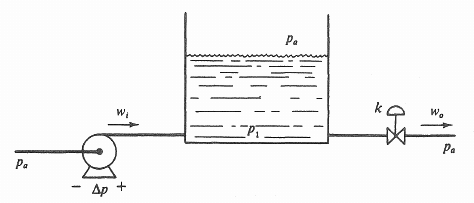
\includegraphics{img/pump_tank_valve.png} donde la bomba presenta la
siguiente característica:
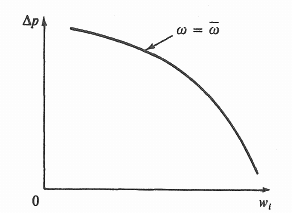
\includegraphics{img/pump_tank_valve_curve.png} - Formule el modelo
matemático, asumiendo que la característica de la bomba corresponde a
una función \(w_i = a_2 \Delta p^2 + a_1 \Delta p + a_0\). - Obtenga el
punto de operación, asumiendo los mismos valores para los parámetros del
ejemplo anterior, y
\(w_i = -7.5 \times 10^{-9} \Delta p^2 + 5 \times 10^{-7} \Delta p + 1 \times 10^{-3}\).
- Simule la respuesta del sistema

    \subsubsection{Solución:}\label{soluciuxf3n}

\begin{itemize}
\tightlist
\item
  La ecuación dinámica del tanque está dada por:
\end{itemize}

    \begin{Verbatim}[commandchars=\\\{\}]
{\color{incolor}In [{\color{incolor}48}]:} \PY{c}{\PYZpc{}\PYZpc{}latex}
         \PY{k}{\PYZbs{}begin}\PY{n+nb}{\PYZob{}}align\PY{n+nb}{\PYZcb{}}
             \PY{k}{\PYZbs{}dot}\PY{n+nb}{\PYZob{}}p\PY{n+nb}{\PYZcb{}}\PY{n+nb}{\PYZus{}}1(t) \PY{n+nb}{\PYZam{}}= \PY{k}{\PYZbs{}frac}\PY{n+nb}{\PYZob{}}\PY{k}{\PYZbs{}rho} g\PY{n+nb}{\PYZcb{}}\PY{n+nb}{\PYZob{}}A\PY{n+nb}{\PYZcb{}}(w\PY{n+nb}{\PYZus{}}i(t) \PYZhy{} w\PY{n+nb}{\PYZus{}}o(t))\PY{k}{\PYZbs{}\PYZbs{}}
             w\PY{n+nb}{\PYZus{}}i(t) \PY{n+nb}{\PYZam{}}= a\PY{n+nb}{\PYZus{}}2(p\PY{n+nb}{\PYZus{}}1(t) \PYZhy{} p\PY{n+nb}{\PYZus{}}a)\PY{n+nb}{\PYZca{}}2 + a\PY{n+nb}{\PYZus{}}1(p\PY{n+nb}{\PYZus{}}1(t) \PYZhy{} p\PY{n+nb}{\PYZus{}}a) + a\PY{n+nb}{\PYZus{}}0\PY{k}{\PYZbs{}\PYZbs{}}
             w\PY{n+nb}{\PYZus{}}o(t) \PY{n+nb}{\PYZam{}}= k \PY{k}{\PYZbs{}sqrt}\PY{n+nb}{\PYZob{}}p\PY{n+nb}{\PYZus{}}1(t) \PYZhy{} p\PY{n+nb}{\PYZus{}}a\PY{n+nb}{\PYZcb{}}
         \PY{k}{\PYZbs{}end}\PY{n+nb}{\PYZob{}}align\PY{n+nb}{\PYZcb{}}
\end{Verbatim}


    \begin{align}
    \dot{p}_1(t) &= \frac{\rho g}{A}(w_i(t) - w_o(t))\\
    w_i(t) &= a_2(p_1(t) - p_a)^2 + a_1(p_1(t) - p_a) + a_0\\
    w_o(t) &= k \sqrt{p_1(t) - p_a}
\end{align}

    
    Reemplazando se obtiene

    \begin{Verbatim}[commandchars=\\\{\}]
{\color{incolor}In [{\color{incolor}49}]:} \PY{c}{\PYZpc{}\PYZpc{}latex}
         \PY{k}{\PYZbs{}begin}\PY{n+nb}{\PYZob{}}equation\PY{n+nb}{\PYZcb{}}
             \PY{k}{\PYZbs{}dot}\PY{n+nb}{\PYZob{}}p\PY{n+nb}{\PYZcb{}}\PY{n+nb}{\PYZus{}}1(t) = \PY{k}{\PYZbs{}frac}\PY{n+nb}{\PYZob{}}\PY{k}{\PYZbs{}rho} g\PY{n+nb}{\PYZcb{}}\PY{n+nb}{\PYZob{}}A\PY{n+nb}{\PYZcb{}}\PY{k}{\PYZbs{}left}(a\PY{n+nb}{\PYZus{}}2(p\PY{n+nb}{\PYZus{}}1(t) \PYZhy{} p\PY{n+nb}{\PYZus{}}a)\PY{n+nb}{\PYZca{}}2 + a\PY{n+nb}{\PYZus{}}1(p\PY{n+nb}{\PYZus{}}1(t) \PYZhy{} p\PY{n+nb}{\PYZus{}}a) + a\PY{n+nb}{\PYZus{}}0 \PYZhy{} k \PY{k}{\PYZbs{}sqrt}\PY{n+nb}{\PYZob{}}p\PY{n+nb}{\PYZus{}}1(t) \PYZhy{} p\PY{n+nb}{\PYZus{}}a\PY{n+nb}{\PYZcb{}}\PY{k}{\PYZbs{}right})
         \PY{k}{\PYZbs{}end}\PY{n+nb}{\PYZob{}}equation\PY{n+nb}{\PYZcb{}}
\end{Verbatim}


    \begin{equation}
    \dot{p}_1(t) = \frac{\rho g}{A}\left(a_2(p_1(t) - p_a)^2 + a_1(p_1(t) - p_a) + a_0 - k \sqrt{p_1(t) - p_a}\right)
\end{equation}

    
    \begin{itemize}
\tightlist
\item
  Para obtener el punto de equilibrio se hace \(\dot{p}_1 = 0\), y se
  despeja \(\bar{p}_1\). Para hacerlo se utiliza la función
  \texttt{fsolve} de la librería \texttt{scipy}. Primero se define la
  función que queremos resolver:
\end{itemize}

    \begin{Verbatim}[commandchars=\\\{\}]
{\color{incolor}In [{\color{incolor}50}]:} \PY{k+kn}{from} \PY{n+nn}{scipy}\PY{n+nn}{.}\PY{n+nn}{optimize} \PY{k}{import} \PY{n}{fsolve}
         \PY{n}{a2} \PY{o}{=} \PY{o}{\PYZhy{}}\PY{l+m+mf}{7.5e\PYZhy{}9}
         \PY{n}{a1} \PY{o}{=} \PY{l+m+mf}{5e\PYZhy{}7}
         \PY{n}{a0} \PY{o}{=} \PY{l+m+mf}{1e\PYZhy{}3}
         \PY{n}{func} \PY{o}{=} \PY{k}{lambda} \PY{n}{p1} \PY{p}{:} \PY{p}{(}\PY{n}{rho}\PY{o}{*}\PY{n}{g}\PY{o}{/}\PY{n}{A}\PY{p}{)}\PY{o}{*}\PY{p}{(}\PY{n}{a2}\PY{o}{*}\PY{p}{(}\PY{n}{p1}\PY{o}{\PYZhy{}}\PY{n}{pa}\PY{p}{)}\PY{o}{*}\PY{o}{*}\PY{l+m+mi}{2} \PY{o}{+} \PY{n}{a1}\PY{o}{*}\PY{p}{(}\PY{n}{p1}\PY{o}{\PYZhy{}}\PY{n}{pa}\PY{p}{)} \PY{o}{+} \PY{n}{a0} \PY{o}{\PYZhy{}} \PY{n}{k}\PY{o}{*}\PY{n}{np}\PY{o}{.}\PY{n}{sqrt}\PY{p}{(}\PY{n}{p1}\PY{o}{\PYZhy{}}\PY{n}{pa}\PY{p}{)}\PY{p}{)}
\end{Verbatim}


    La función \texttt{fsolve} busca de manera iterativa la solución, por lo
que requiere de un valor inicial. Dicho valor puede obtenerse graficando
la función en un intervalo apropiado y seleccionando un valor de \(p_1\)
cercano al cruce por cero:

    \begin{Verbatim}[commandchars=\\\{\}]
{\color{incolor}In [{\color{incolor}51}]:} \PY{n}{p1} \PY{o}{=} \PY{n}{np}\PY{o}{.}\PY{n}{linspace}\PY{p}{(}\PY{n}{pa}\PY{p}{,}\PY{n}{pa}\PY{o}{+}\PY{l+m+mi}{400}\PY{p}{,}\PY{l+m+mi}{201}\PY{p}{)}
         \PY{n}{plt}\PY{o}{.}\PY{n}{plot}\PY{p}{(}\PY{n}{p1}\PY{p}{,}\PY{n}{func}\PY{p}{(}\PY{n}{p1}\PY{p}{)}\PY{p}{)}
         \PY{n}{plt}\PY{o}{.}\PY{n}{xlabel}\PY{p}{(}\PY{l+s+sa}{r}\PY{l+s+s2}{\PYZdq{}}\PY{l+s+s2}{\PYZdl{}p\PYZus{}1\PYZdl{}}\PY{l+s+s2}{\PYZdq{}}\PY{p}{,}\PY{n}{fontsize}\PY{o}{=}\PY{l+m+mi}{20}\PY{p}{)}
         \PY{n}{plt}\PY{o}{.}\PY{n}{ylabel}\PY{p}{(}\PY{l+s+sa}{r}\PY{l+s+s2}{\PYZdq{}}\PY{l+s+s2}{func}\PY{l+s+s2}{\PYZdq{}}\PY{p}{,}\PY{n}{fontsize}\PY{o}{=}\PY{l+m+mi}{20}\PY{p}{)}
         \PY{n}{plt}\PY{o}{.}\PY{n}{grid}\PY{p}{(}\PY{p}{)}
         \PY{n}{plt}\PY{o}{.}\PY{n}{show}\PY{p}{(}\PY{p}{)}
\end{Verbatim}


    \begin{center}
    \adjustimage{max size={0.9\linewidth}{0.9\paperheight}}{output_102_0.png}
    \end{center}
    { \hspace*{\fill} \\}
    
    Ahora se resuelve la ecuación usando la función \texttt{fsolve}:

    \begin{Verbatim}[commandchars=\\\{\}]
{\color{incolor}In [{\color{incolor}52}]:} \PY{n}{p1\PYZus{}initial} \PY{o}{=} \PY{l+m+mi}{101500}
         \PY{n}{p1\PYZus{}soln} \PY{o}{=} \PY{n}{fsolve}\PY{p}{(}\PY{n}{func}\PY{p}{,} \PY{n}{p1\PYZus{}initial}\PY{p}{)}
         \PY{n}{deltapbar} \PY{o}{=} \PY{n}{p1\PYZus{}soln}\PY{o}{\PYZhy{}}\PY{n}{pa}
         \PY{n}{wi\PYZus{}bar} \PY{o}{=} \PY{n}{a2}\PY{o}{*}\PY{p}{(}\PY{n}{p1\PYZus{}soln}\PY{o}{\PYZhy{}}\PY{n}{pa}\PY{p}{)}\PY{o}{*}\PY{o}{*}\PY{l+m+mi}{2} \PY{o}{+} \PY{n}{a1}\PY{o}{*}\PY{p}{(}\PY{n}{p1\PYZus{}soln}\PY{o}{\PYZhy{}}\PY{n}{pa}\PY{p}{)} \PY{o}{+} \PY{n}{a0}
         \PY{n+nb}{print}\PY{p}{(}\PY{n}{deltapbar}\PY{p}{)}
         \PY{n+nb}{print}\PY{p}{(}\PY{n}{wi\PYZus{}bar}\PY{p}{)}
\end{Verbatim}


    \begin{Verbatim}[commandchars=\\\{\}]
[221.19766661]
[0.00074364]

    \end{Verbatim}

    Al graficar las curvas características para la válvula y la bomba se
observa que el punto de equilibrio corresponde a la intersección de las
dos curvas:

    \begin{Verbatim}[commandchars=\\\{\}]
{\color{incolor}In [{\color{incolor}53}]:} \PY{n}{deltap} \PY{o}{=} \PY{n}{np}\PY{o}{.}\PY{n}{linspace}\PY{p}{(}\PY{l+m+mf}{0.0}\PY{p}{,}\PY{l+m+mi}{500}\PY{p}{,}\PY{l+m+mi}{100}\PY{p}{)}
         \PY{n}{w\PYZus{}v} \PY{o}{=} \PY{n}{k}\PY{o}{*}\PY{n}{np}\PY{o}{.}\PY{n}{sqrt}\PY{p}{(}\PY{n}{deltap}\PY{p}{)}
         \PY{n}{plt}\PY{o}{.}\PY{n}{plot}\PY{p}{(}\PY{n}{w\PYZus{}v}\PY{p}{,}\PY{n}{deltap}\PY{p}{,}\PY{n}{label}\PY{o}{=}\PY{l+s+s1}{\PYZsq{}}\PY{l+s+s1}{Valvula}\PY{l+s+s1}{\PYZsq{}}\PY{p}{)}
         \PY{n}{w\PYZus{}p} \PY{o}{=} \PY{o}{\PYZhy{}}\PY{l+m+mf}{7.5e\PYZhy{}9}\PY{o}{*}\PY{n}{deltap}\PY{o}{*}\PY{o}{*}\PY{l+m+mi}{2} \PY{o}{+} \PY{l+m+mf}{5e\PYZhy{}7}\PY{o}{*}\PY{n}{deltap} \PY{o}{+} \PY{l+m+mf}{1e\PYZhy{}3}
         \PY{n}{plt}\PY{o}{.}\PY{n}{plot}\PY{p}{(}\PY{n}{w\PYZus{}p}\PY{p}{,}\PY{n}{deltap}\PY{p}{,}\PY{n}{label}\PY{o}{=}\PY{l+s+s1}{\PYZsq{}}\PY{l+s+s1}{Bomba}\PY{l+s+s1}{\PYZsq{}}\PY{p}{)}
         \PY{n}{plt}\PY{o}{.}\PY{n}{plot}\PY{p}{(}\PY{n}{wi\PYZus{}bar}\PY{p}{,}\PY{n}{deltapbar}\PY{p}{,} \PY{n}{marker}\PY{o}{=}\PY{l+s+s1}{\PYZsq{}}\PY{l+s+s1}{o}\PY{l+s+s1}{\PYZsq{}}\PY{p}{,} \PY{n}{markersize}\PY{o}{=}\PY{l+m+mi}{10}\PY{p}{,} \PY{n}{color}\PY{o}{=}\PY{l+s+s1}{\PYZsq{}}\PY{l+s+s1}{red}\PY{l+s+s1}{\PYZsq{}}\PY{p}{)}
         \PY{n}{plt}\PY{o}{.}\PY{n}{xlabel}\PY{p}{(}\PY{l+s+sa}{r}\PY{l+s+s2}{\PYZdq{}}\PY{l+s+s2}{\PYZdl{}w\PYZdl{}}\PY{l+s+s2}{\PYZdq{}}\PY{p}{,}\PY{n}{fontsize}\PY{o}{=}\PY{l+m+mi}{20}\PY{p}{)}
         \PY{n}{plt}\PY{o}{.}\PY{n}{ylabel}\PY{p}{(}\PY{l+s+s2}{\PYZdq{}}\PY{l+s+s2}{\PYZdl{}}\PY{l+s+s2}{\PYZbs{}}\PY{l+s+s2}{Delta p\PYZdl{}}\PY{l+s+s2}{\PYZdq{}}\PY{p}{,}\PY{n}{fontsize}\PY{o}{=}\PY{l+m+mi}{20}\PY{p}{)}
         \PY{n}{plt}\PY{o}{.}\PY{n}{legend}\PY{p}{(}\PY{n}{loc}\PY{o}{=}\PY{l+s+s1}{\PYZsq{}}\PY{l+s+s1}{upper left}\PY{l+s+s1}{\PYZsq{}}\PY{p}{,}\PY{n}{fontsize}\PY{o}{=}\PY{l+m+mi}{20}\PY{p}{)}
         \PY{n}{plt}\PY{o}{.}\PY{n}{xlim}\PY{p}{(}\PY{l+m+mi}{0}\PY{p}{,}\PY{l+m+mf}{0.001}\PY{p}{)}
         \PY{n}{plt}\PY{o}{.}\PY{n}{ylim}\PY{p}{(}\PY{l+m+mi}{0}\PY{p}{,}\PY{l+m+mi}{500}\PY{p}{)}
\end{Verbatim}


\begin{Verbatim}[commandchars=\\\{\}]
{\color{outcolor}Out[{\color{outcolor}53}]:} (0, 500)
\end{Verbatim}
            
    \begin{center}
    \adjustimage{max size={0.9\linewidth}{0.9\paperheight}}{output_106_1.png}
    \end{center}
    { \hspace*{\fill} \\}
    
    \begin{itemize}
\tightlist
\item
  Para simular la respuesta del sistema se utiliza la misma estrategia
  que en el ejemplo anterior.
\end{itemize}

    \begin{Verbatim}[commandchars=\\\{\}]
{\color{incolor}In [{\color{incolor}54}]:} \PY{k}{def} \PY{n+nf}{hydrsys2\PYZus{}eq}\PY{p}{(}\PY{n}{t}\PY{p}{,} \PY{n}{p1}\PY{p}{)}\PY{p}{:}    
             \PY{n}{A} \PY{o}{=} \PY{l+m+mi}{2}
             \PY{n}{rho} \PY{o}{=} \PY{l+m+mi}{1000}
             \PY{n}{k} \PY{o}{=} \PY{l+m+mf}{5e\PYZhy{}5}
             \PY{n}{pa} \PY{o}{=} \PY{l+m+mf}{1.013e5}
             \PY{n}{g} \PY{o}{=} \PY{l+m+mf}{9.807}
             \PY{n}{a2} \PY{o}{=} \PY{o}{\PYZhy{}}\PY{l+m+mf}{7.5e\PYZhy{}9}
             \PY{n}{a1} \PY{o}{=} \PY{l+m+mf}{5e\PYZhy{}7}
             \PY{n}{a0} \PY{o}{=} \PY{l+m+mf}{1e\PYZhy{}3}
             \PY{n}{pdot} \PY{o}{=} \PY{p}{(}\PY{n}{rho}\PY{o}{*}\PY{n}{g}\PY{o}{/}\PY{n}{A}\PY{p}{)}\PY{o}{*}\PY{p}{(}\PY{n}{a2}\PY{o}{*}\PY{p}{(}\PY{n}{p1}\PY{o}{\PYZhy{}}\PY{n}{pa}\PY{p}{)}\PY{o}{*}\PY{o}{*}\PY{l+m+mi}{2} \PY{o}{+} \PY{n}{a1}\PY{o}{*}\PY{p}{(}\PY{n}{p1}\PY{o}{\PYZhy{}}\PY{n}{pa}\PY{p}{)} \PY{o}{+} \PY{n}{a0} \PY{o}{\PYZhy{}} \PY{n}{k}\PY{o}{*}\PY{n}{math}\PY{o}{.}\PY{n}{sqrt}\PY{p}{(}\PY{n}{p1}\PY{o}{\PYZhy{}}\PY{n}{pa}\PY{p}{)}\PY{p}{)}
             \PY{k}{return} \PY{n}{pdot}
\end{Verbatim}


    Ahora, implementamos el método iterativo de Runge-Kutta de dos etapas:

    \begin{Verbatim}[commandchars=\\\{\}]
{\color{incolor}In [{\color{incolor}55}]:} \PY{n}{tf} \PY{o}{=} \PY{l+m+mi}{1000}
         \PY{n}{N} \PY{o}{=} \PY{l+m+mi}{10000}
         \PY{n}{h} \PY{o}{=} \PY{n}{tf}\PY{o}{/}\PY{n}{N}
         \PY{n}{t} \PY{o}{=} \PY{n}{np}\PY{o}{.}\PY{n}{linspace}\PY{p}{(}\PY{l+m+mf}{0.0}\PY{p}{,}\PY{n}{tf}\PY{p}{,}\PY{n}{num}\PY{o}{=}\PY{n}{N}\PY{p}{)}
         \PY{n}{p1} \PY{o}{=} \PY{n}{np}\PY{o}{.}\PY{n}{zeros}\PY{p}{(}\PY{n}{N}\PY{p}{)}
         \PY{n}{p1}\PY{p}{[}\PY{l+m+mi}{0}\PY{p}{]} \PY{o}{=} \PY{n}{pa}
         \PY{k}{for} \PY{n}{i} \PY{o+ow}{in} \PY{n+nb}{range}\PY{p}{(}\PY{l+m+mi}{0}\PY{p}{,}\PY{n}{N}\PY{o}{\PYZhy{}}\PY{l+m+mi}{1}\PY{p}{)}\PY{p}{:}
             \PY{n}{k1} \PY{o}{=} \PY{n}{hydrsys2\PYZus{}eq}\PY{p}{(}\PY{n}{t}\PY{p}{[}\PY{n}{i}\PY{p}{]}\PY{p}{,}\PY{n}{p1}\PY{p}{[}\PY{n}{i}\PY{p}{]}\PY{p}{)}
             \PY{n}{k2} \PY{o}{=} \PY{n}{hydrsys2\PYZus{}eq}\PY{p}{(}\PY{n}{t}\PY{p}{[}\PY{n}{i}\PY{p}{]}\PY{o}{+}\PY{l+m+mf}{0.5}\PY{o}{*}\PY{n}{h}\PY{p}{,}\PY{n}{p1}\PY{p}{[}\PY{n}{i}\PY{p}{]}\PY{o}{+}\PY{l+m+mf}{0.5}\PY{o}{*}\PY{n}{h}\PY{o}{*}\PY{n}{k1}\PY{p}{)}
             \PY{n}{p1}\PY{p}{[}\PY{n}{i}\PY{o}{+}\PY{l+m+mi}{1}\PY{p}{]} \PY{o}{=} \PY{n}{p1}\PY{p}{[}\PY{n}{i}\PY{p}{]} \PY{o}{+} \PY{n}{h}\PY{o}{*}\PY{n}{k2}
\end{Verbatim}


    Finalmente graficamos la respuesta:

    \begin{Verbatim}[commandchars=\\\{\}]
{\color{incolor}In [{\color{incolor}56}]:} \PY{n}{p1bar} \PY{o}{=} \PY{n}{p1\PYZus{}soln}\PY{o}{*}\PY{n}{np}\PY{o}{.}\PY{n}{ones}\PY{p}{(}\PY{n}{N}\PY{p}{)}
         \PY{n}{plt}\PY{o}{.}\PY{n}{plot}\PY{p}{(}\PY{n}{t}\PY{p}{,}\PY{n}{p1}\PY{p}{,}\PY{l+s+s1}{\PYZsq{}}\PY{l+s+s1}{b}\PY{l+s+s1}{\PYZsq{}}\PY{p}{,}\PY{n}{label}\PY{o}{=}\PY{l+s+sa}{r}\PY{l+s+s2}{\PYZdq{}}\PY{l+s+s2}{\PYZdl{}p\PYZus{}1\PYZdl{}}\PY{l+s+s2}{\PYZdq{}}\PY{p}{)}
         \PY{n}{plt}\PY{o}{.}\PY{n}{plot}\PY{p}{(}\PY{n}{t}\PY{p}{,}\PY{n}{p1bar}\PY{p}{,}\PY{l+s+s1}{\PYZsq{}}\PY{l+s+s1}{r\PYZhy{}\PYZhy{}}\PY{l+s+s1}{\PYZsq{}}\PY{p}{,}\PY{n}{label}\PY{o}{=}\PY{l+s+sa}{r}\PY{l+s+s2}{\PYZdq{}}\PY{l+s+s2}{\PYZdl{}}\PY{l+s+s2}{\PYZbs{}}\PY{l+s+s2}{bar}\PY{l+s+si}{\PYZob{}p\PYZcb{}}\PY{l+s+s2}{\PYZus{}1\PYZdl{}}\PY{l+s+s2}{\PYZdq{}}\PY{p}{)}
         \PY{n}{plt}\PY{o}{.}\PY{n}{title}\PY{p}{(}\PY{l+s+s2}{\PYZdq{}}\PY{l+s+s2}{Respuesta paso}\PY{l+s+s2}{\PYZdq{}}\PY{p}{,}\PY{n}{fontsize}\PY{o}{=}\PY{l+m+mi}{20}\PY{p}{)}
         \PY{n}{plt}\PY{o}{.}\PY{n}{xlabel}\PY{p}{(}\PY{l+s+sa}{r}\PY{l+s+s2}{\PYZdq{}}\PY{l+s+s2}{Tiempo [s]}\PY{l+s+s2}{\PYZdq{}}\PY{p}{,}\PY{n}{fontsize}\PY{o}{=}\PY{l+m+mi}{20}\PY{p}{)}
         \PY{n}{plt}\PY{o}{.}\PY{n}{ylabel}\PY{p}{(}\PY{l+s+sa}{r}\PY{l+s+s2}{\PYZdq{}}\PY{l+s+s2}{\PYZdl{}p\PYZus{}1\PYZdl{}}\PY{l+s+s2}{\PYZdq{}}\PY{p}{,}\PY{n}{fontsize}\PY{o}{=}\PY{l+m+mi}{20}\PY{p}{)}
         \PY{n}{plt}\PY{o}{.}\PY{n}{legend}\PY{p}{(}\PY{n}{loc}\PY{o}{=}\PY{l+s+s1}{\PYZsq{}}\PY{l+s+s1}{center right}\PY{l+s+s1}{\PYZsq{}}\PY{p}{,}\PY{n}{fontsize}\PY{o}{=}\PY{l+m+mi}{20}\PY{p}{)}
\end{Verbatim}


\begin{Verbatim}[commandchars=\\\{\}]
{\color{outcolor}Out[{\color{outcolor}56}]:} <matplotlib.legend.Legend at 0x7f9d2dd1eda0>
\end{Verbatim}
            
    \begin{center}
    \adjustimage{max size={0.9\linewidth}{0.9\paperheight}}{output_112_1.png}
    \end{center}
    { \hspace*{\fill} \\}
    
    En la figura se observa que el sistema se estabiliza en el valor de
equilibrio calculado anteriormente.

    \subsubsection{Ejercicio:}\label{ejercicio}

Dado el sistema mostrado en la figura:
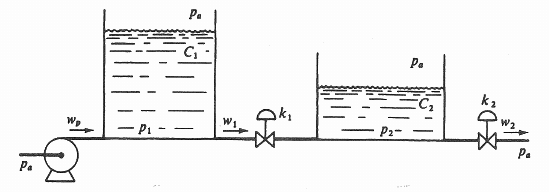
\includegraphics{img/pump_2tanks_2valves.png} - Formule el modelo
matemático, asumiendo que la característica de la bomba corresponde a
una función \(w_i = a_2 \Delta p^2 + a_1 \Delta p + a_0\). - Obtenga el
punto de operación, asumiendo los siguientes valores para los
parámetros: \(A_1=2\), \(A_2=3\), \(\rho=1000\),
\(k_1 = 3 \times 10^{-5}\), \(k_2 = 5 \times 10^{-5}\),
\(p_a = 1.013 \times 10^{5}\), \(g = 9.807\),
\(w_p = -7.5 \times 10^{-9} \Delta p^2 + 5 \times 10^{-7} \Delta p + 1 \times 10^{-3}\).

\begin{itemize}
\tightlist
\item
  Simule la respuesta del sistema
\end{itemize}

    \subsection{References}\label{references}

\begin{itemize}
\tightlist
\item
  Close, C., Frederick, D., Newell, J.
  \href{https://books.google.com.co/books?isbn=0471452963}{Modeling and
  Analysis of Dynamic Systems}. 3rd Edition. Jonh Wiley \& Sons, 2002.
\end{itemize}


    % Add a bibliography block to the postdoc
    
    
    
    \end{document}
